\documentclass{article}
\usepackage{davidcorzo}
\preliminaries{Ensayo de costos - Visita a Xamán}{2020-Mar-02}{David Gabriel Corzo Mcmath}

%%%%%%%%%%%%%%%%%%%%%%%%%%%%%%%%%%%%%%%%%%%%%%%%%%%%%%%%%%%%%%%%%%%%%%%%%%%%%%%%%%%%%%%%%%%%%%%%%%%%%%%%%%%%%%%%%%%%%%%%%%%%%%%%%%%%%%%%%%%%%%%
\begin{document}
\maketitle

\tikzblockdefinitions

\section{Visita a la empresa Xamán}
Xamán es una empresa que se dedica a la producción de cerveza artesanal, entre las cosas interesantes que se pudo absorber de la visita a dicha empresa fue el proceso de la cerveza y las distintas formas de elaborarla. 


%----------------------------------------------------------------------------------------
\subsection{Extra: Proceso de elaboración de la cerveza}
\begin{center}    
    \begin{tikzpicture}[node distance = 4cm, auto]
        \node [block] (1) {1. Filtro de agua}; 
        \node [block,right of=1] (2) {2. Molino }; 
        \node [block,right of=2] (3) {3. El tanque de maseración}; 
        \node [block,right of=3] (4) {4. Boiling tank}; 
        \node [block,below of=4, node distance = 2cm,auto] (5) {5. Tanque de fermentación}; 
        \node [block,left of=5] (6) {6. Filtrado}; 
        \node [block,left of=6] (7) {7. Carbonatación}; 
        \node [block,left of=7] (8) {8. Empaquetado}; 

        \path [line] (1) -- (2);
        \path [line] (2) -- (3);
        \path [line] (3) -- (4);
        \path [line] (4) -- (5);
        \path [line] (5) -- (6);
        \path [line] (6) -- (7);
        \path [line] (7) -- (8);

    \end{tikzpicture}
\end{center}

%%%%%%%%%%%%%%%%%%%%%%%%%%%%%%%%%%%%%%%%%%%%%%%%%%%%%%%%%%%%%%%%%%%%%%%%%%%%%%%%%%%%%%%%%%
\section{Costos y análisis económico}
El tour de la planta de producción fue dada por uno de los fundadores de la empresa, él en su presentación comentaba al grupo acerca de las altas barreras de entrada al negocio. Dado a la necesidad de licencias sanitarias y el tiempo que se toma en aprobarlas es tardado el proceso de entrar al negocio, en el caso de Xamán se tardo un tiempo récord de un poco más de un año.

\begin{center}
   \begin{longtable}{ | p{4.5cm} | p{11.5cm} | }
       \hline
            \textbf{Costos Variables: }  & 
            \begin{itemize}
                \item 
            \end{itemize} \\ 

       \hline
            \textbf{Costos fijos: } & 
            \begin{itemize}
                \item 
            \end{itemize} \\ 
            
        \hline
            \textbf{Costos Marginales: } & 
            \begin{itemize}
                \item 
            \end{itemize} \\ 
            
        \hline
            \textbf{Costos irrecuperables: } & 
            \begin{itemize}
                \item 
            \end{itemize} \\ 
        \hline
        
        \hline
            \textbf{Rendimientos de escala: } & 
            \begin{itemize}
                \item 
            \end{itemize} \\ 
        \hline
        
        \hline
            \textbf{Economías de escala: } & 
            \begin{itemize}
                \item 
            \end{itemize} \\ 
        \hline
        
        \hline
            \textbf{Economías de alcance: } & 
            \begin{itemize}
                \item 
            \end{itemize} \\ 
        \hline
        
        \hline
            \textbf{Factores de producción: } & 
            \begin{itemize}
                \item 
            \end{itemize} \\ 
        \hline
        
        \hline
            \textbf{Precio de producción: } & 
            \begin{itemize}
                \item 
            \end{itemize} \\ 
        \hline
        
        \hline
            \textbf{Tiempo: } & 
            \begin{itemize}
                \item 
            \end{itemize}  \\ 
        \hline
        
   \end{longtable}
\end{center}




%%%%%%%%%%%%%%%%%%%%%%%%%%%%%%%%%%%%%%%%%%%%%%%%%%%%%%%%%%%%%%%%%%%%%%%%%%%%%%%%%%%%%%%%%%
\section{Fotos}
\begin{figure}[htbp]
    \centering
    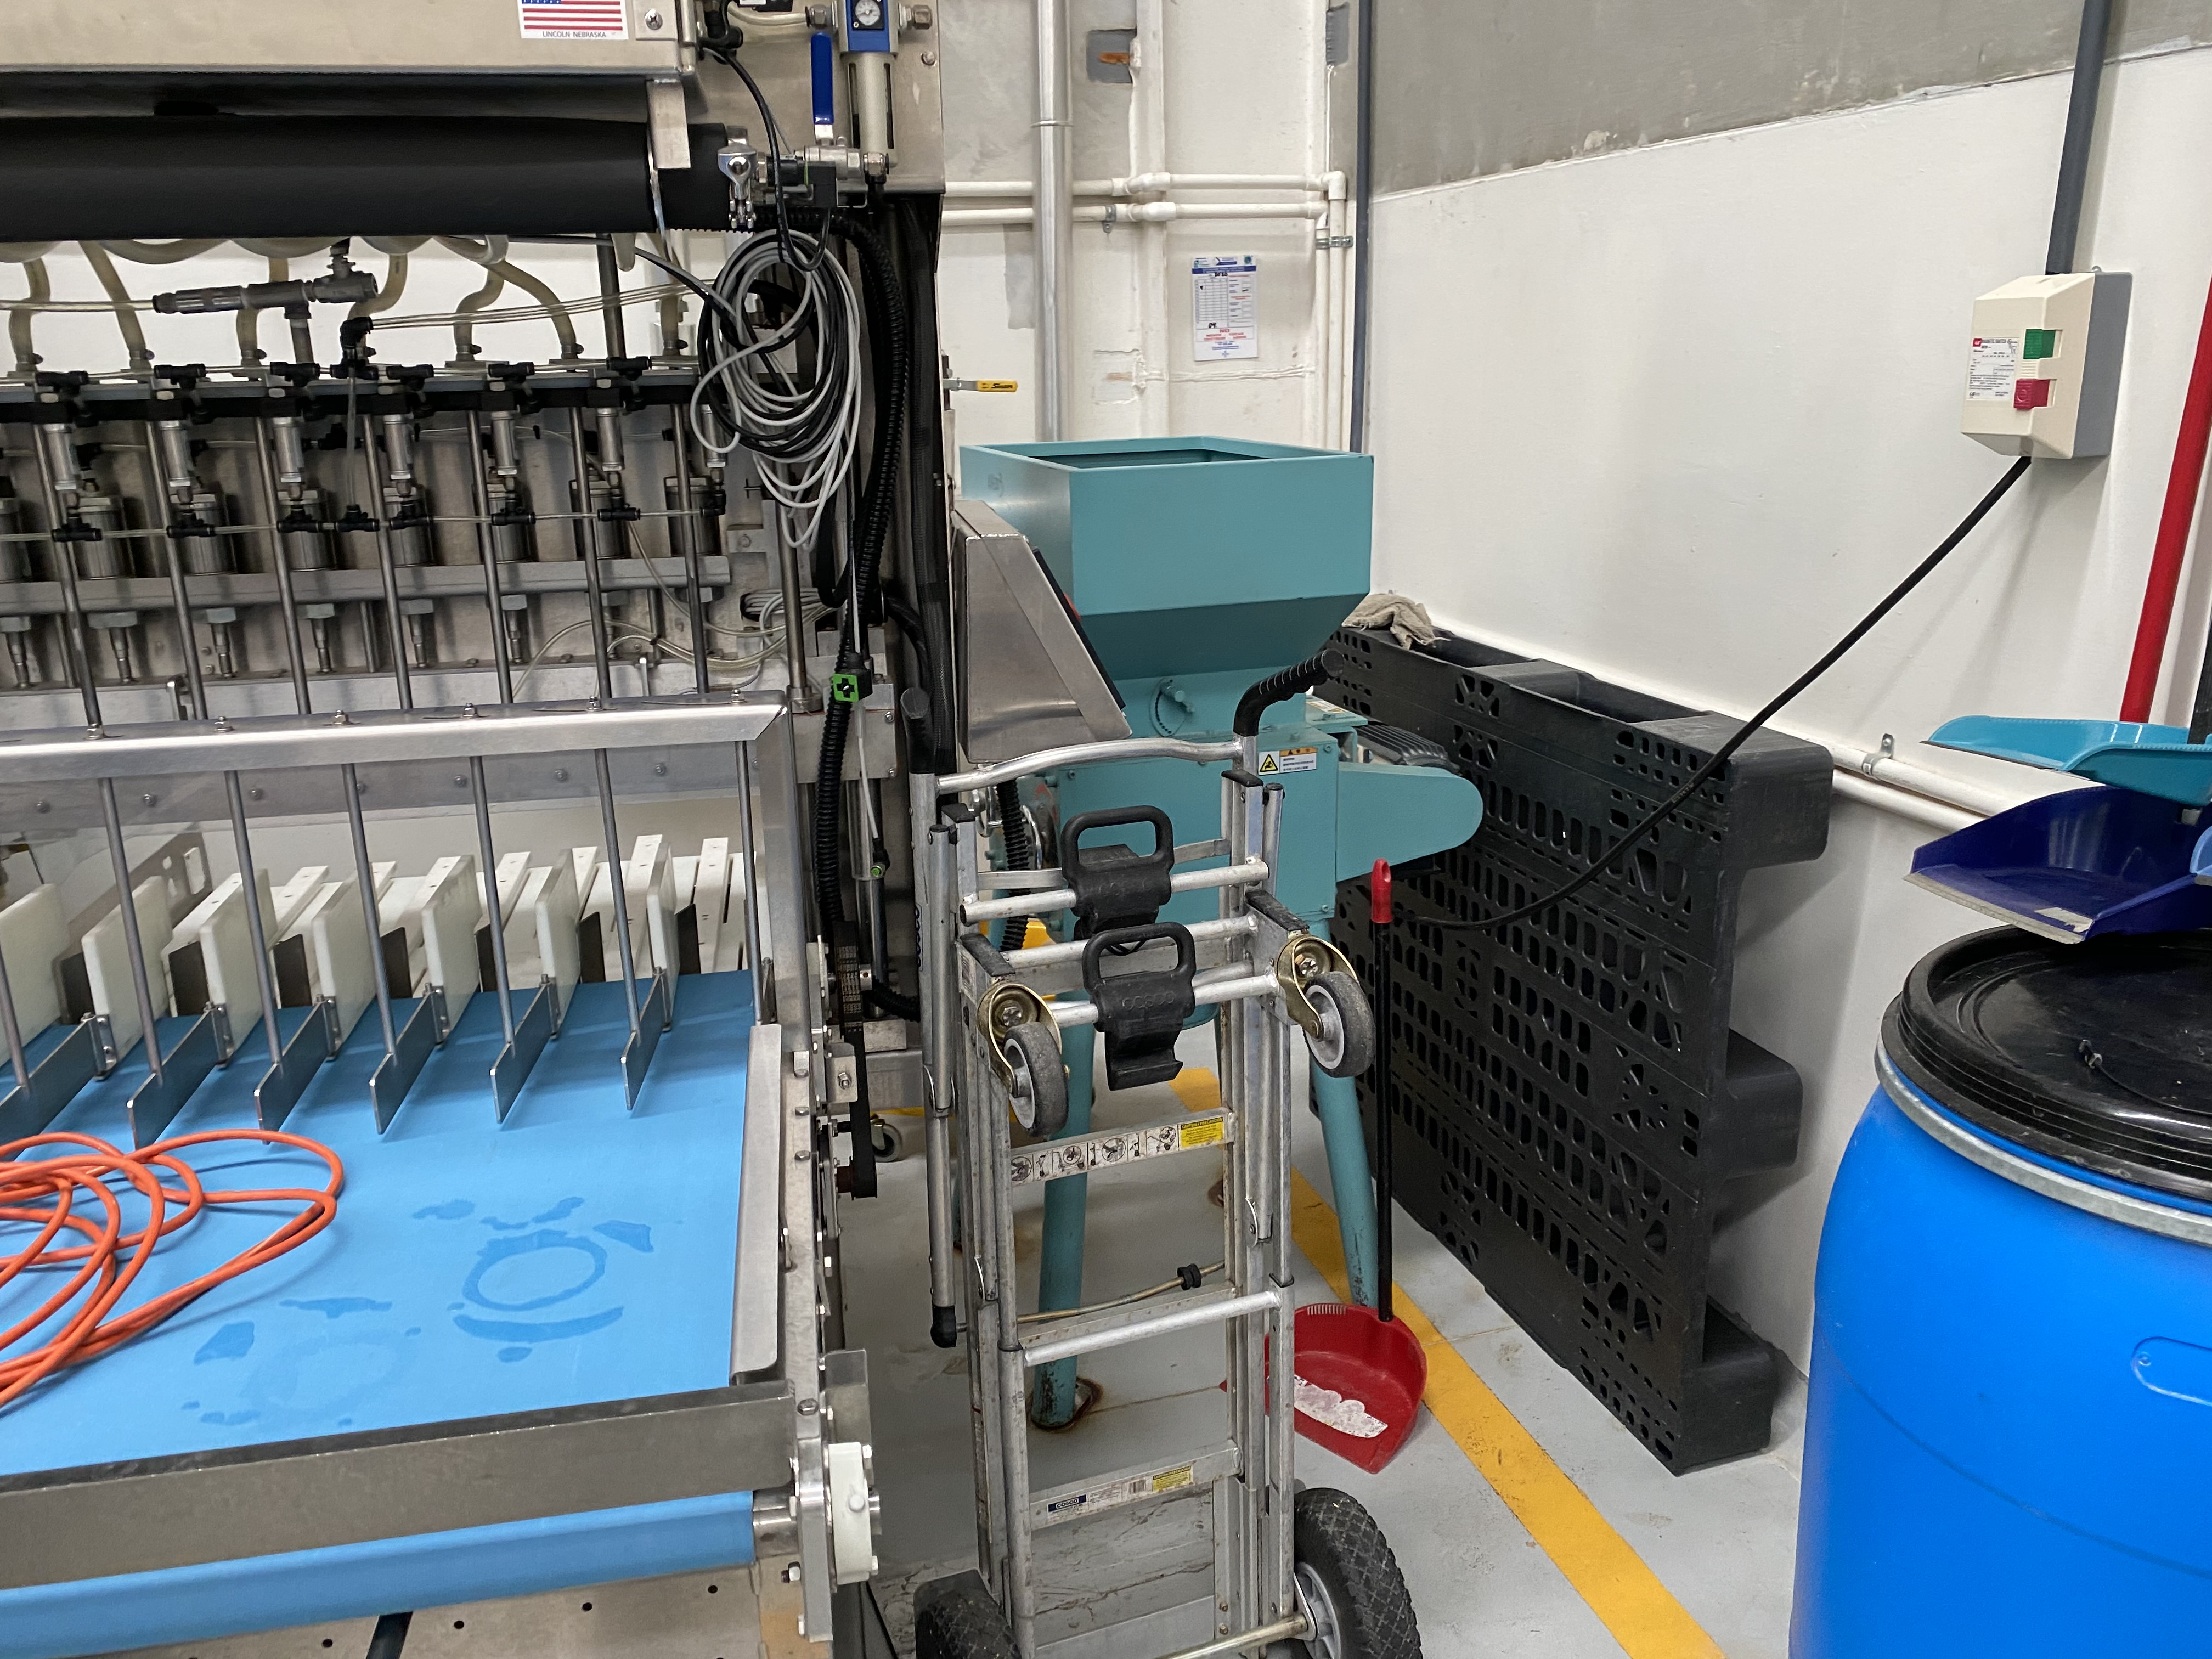
\includegraphics[width=8cm]{./img/IMG-7090.JPG}
    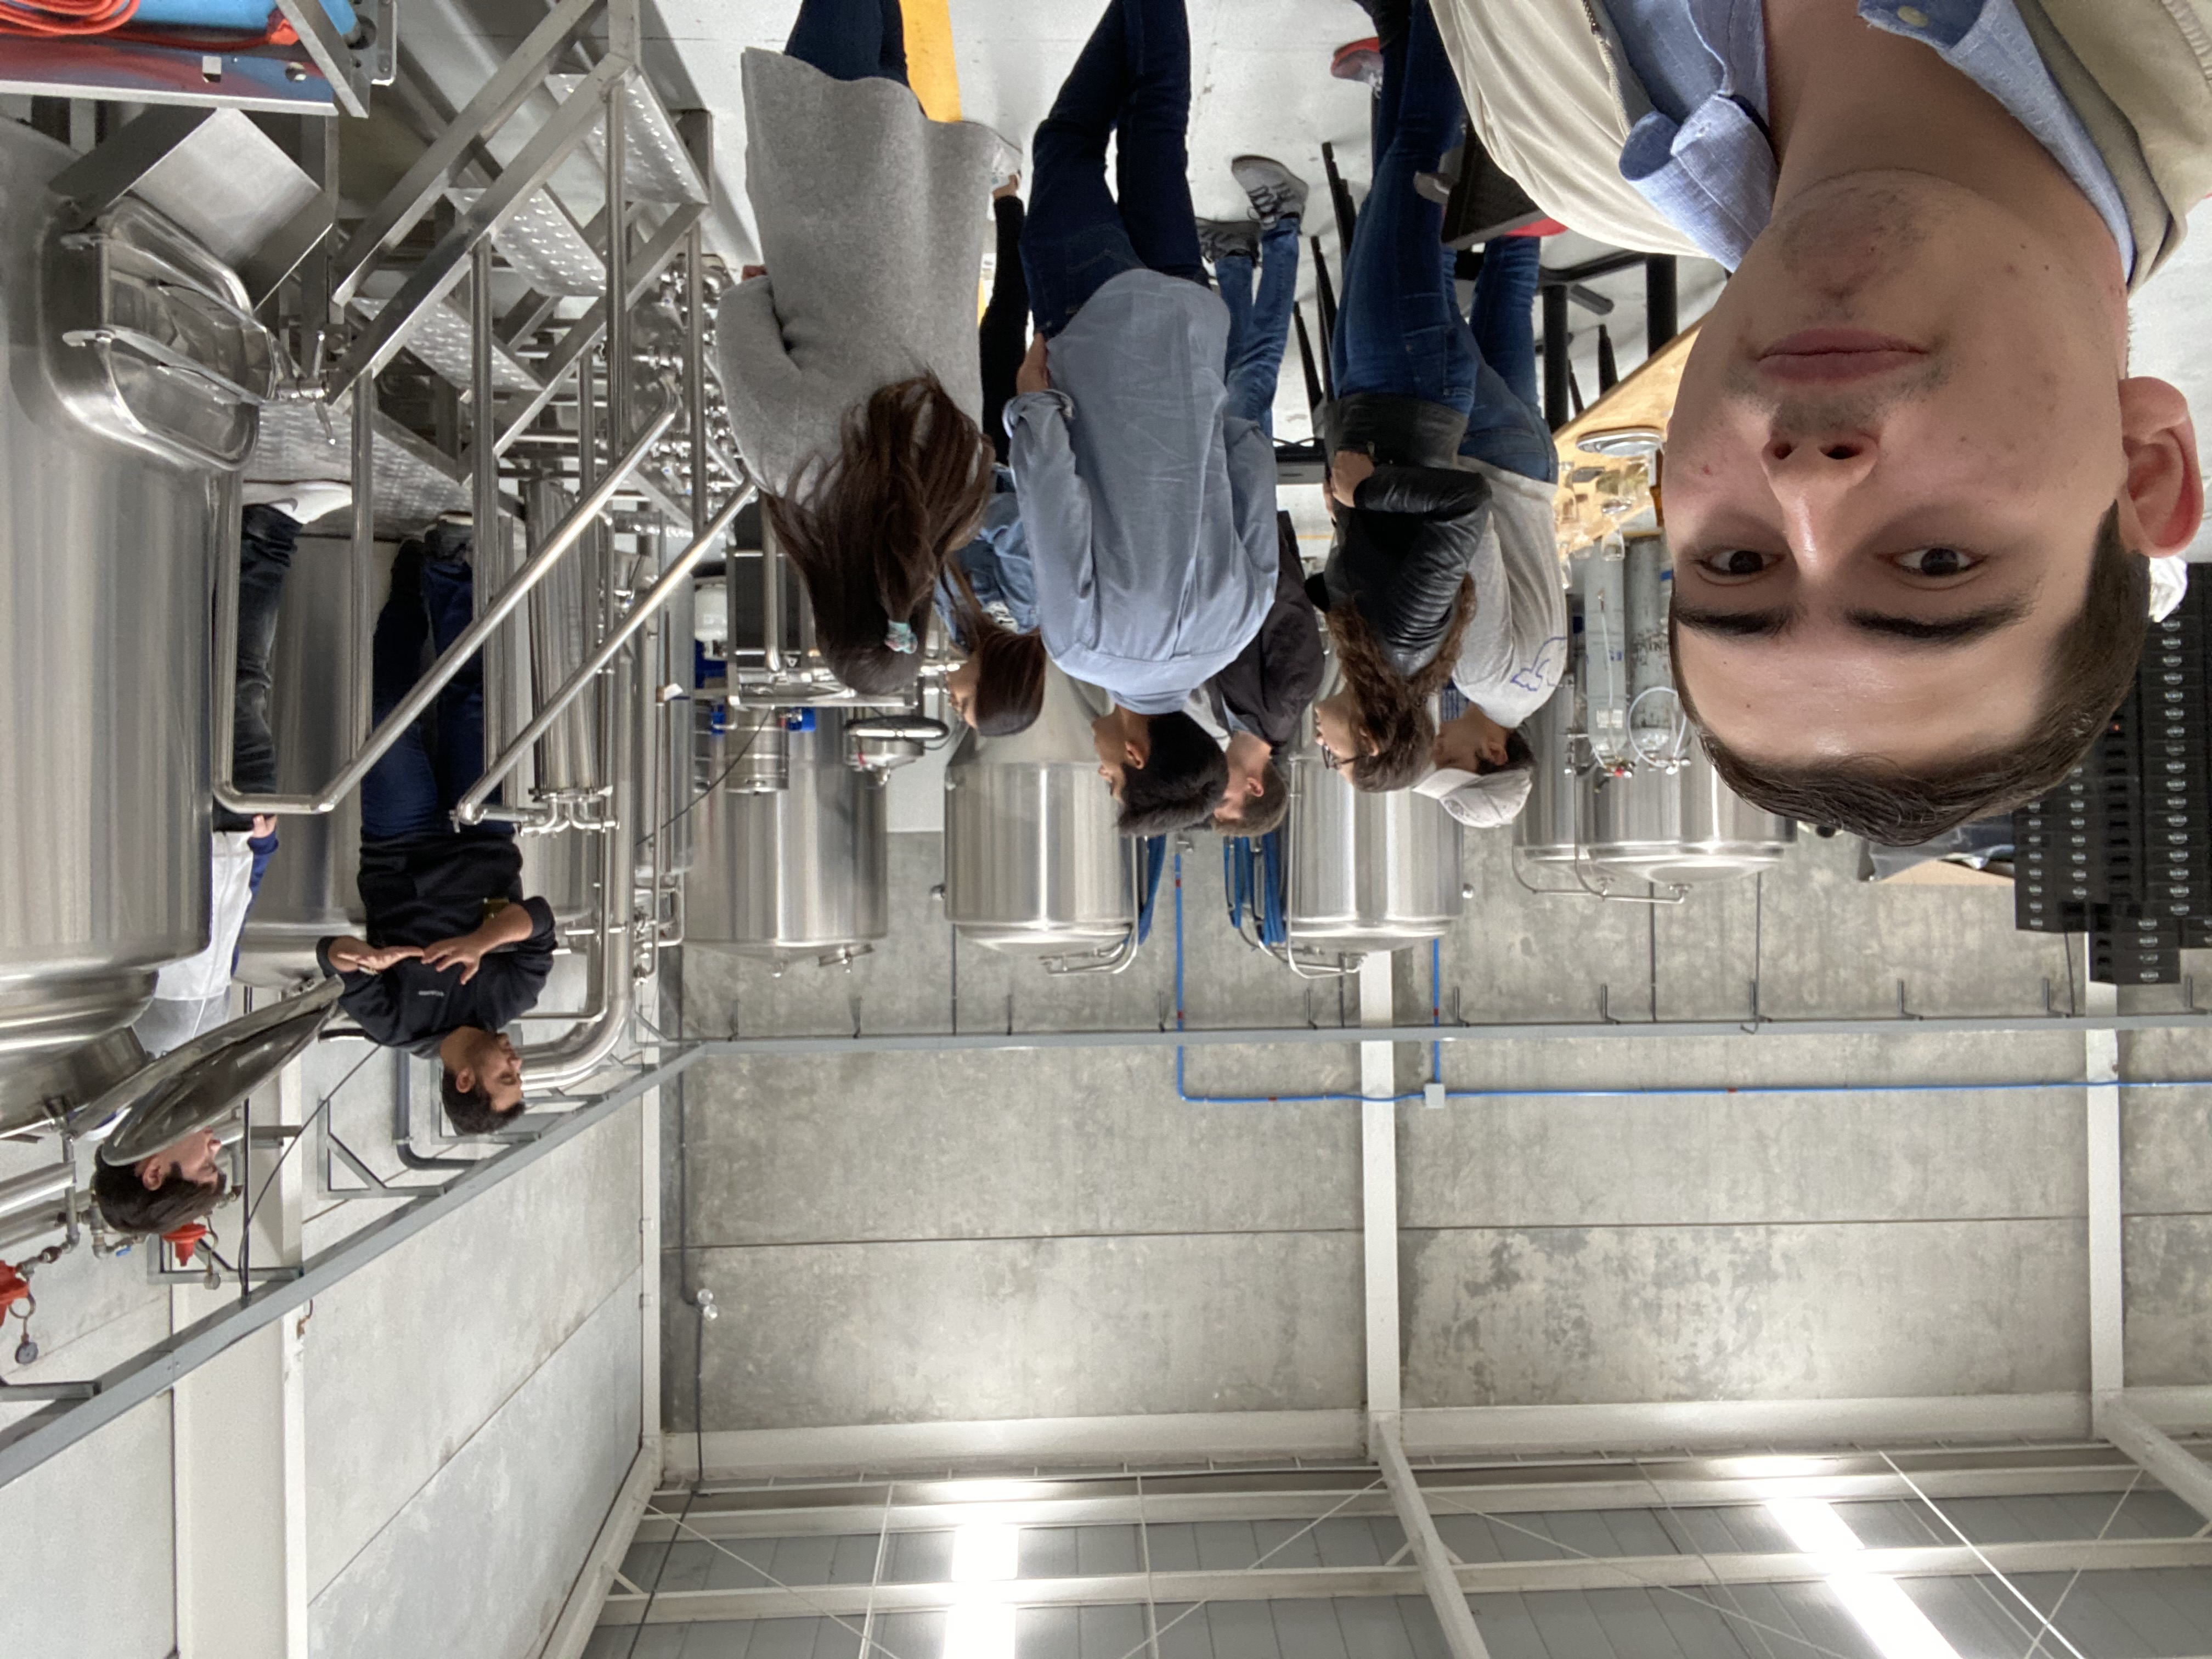
\includegraphics[width=8cm]{./img/IMG-7091.JPG}
    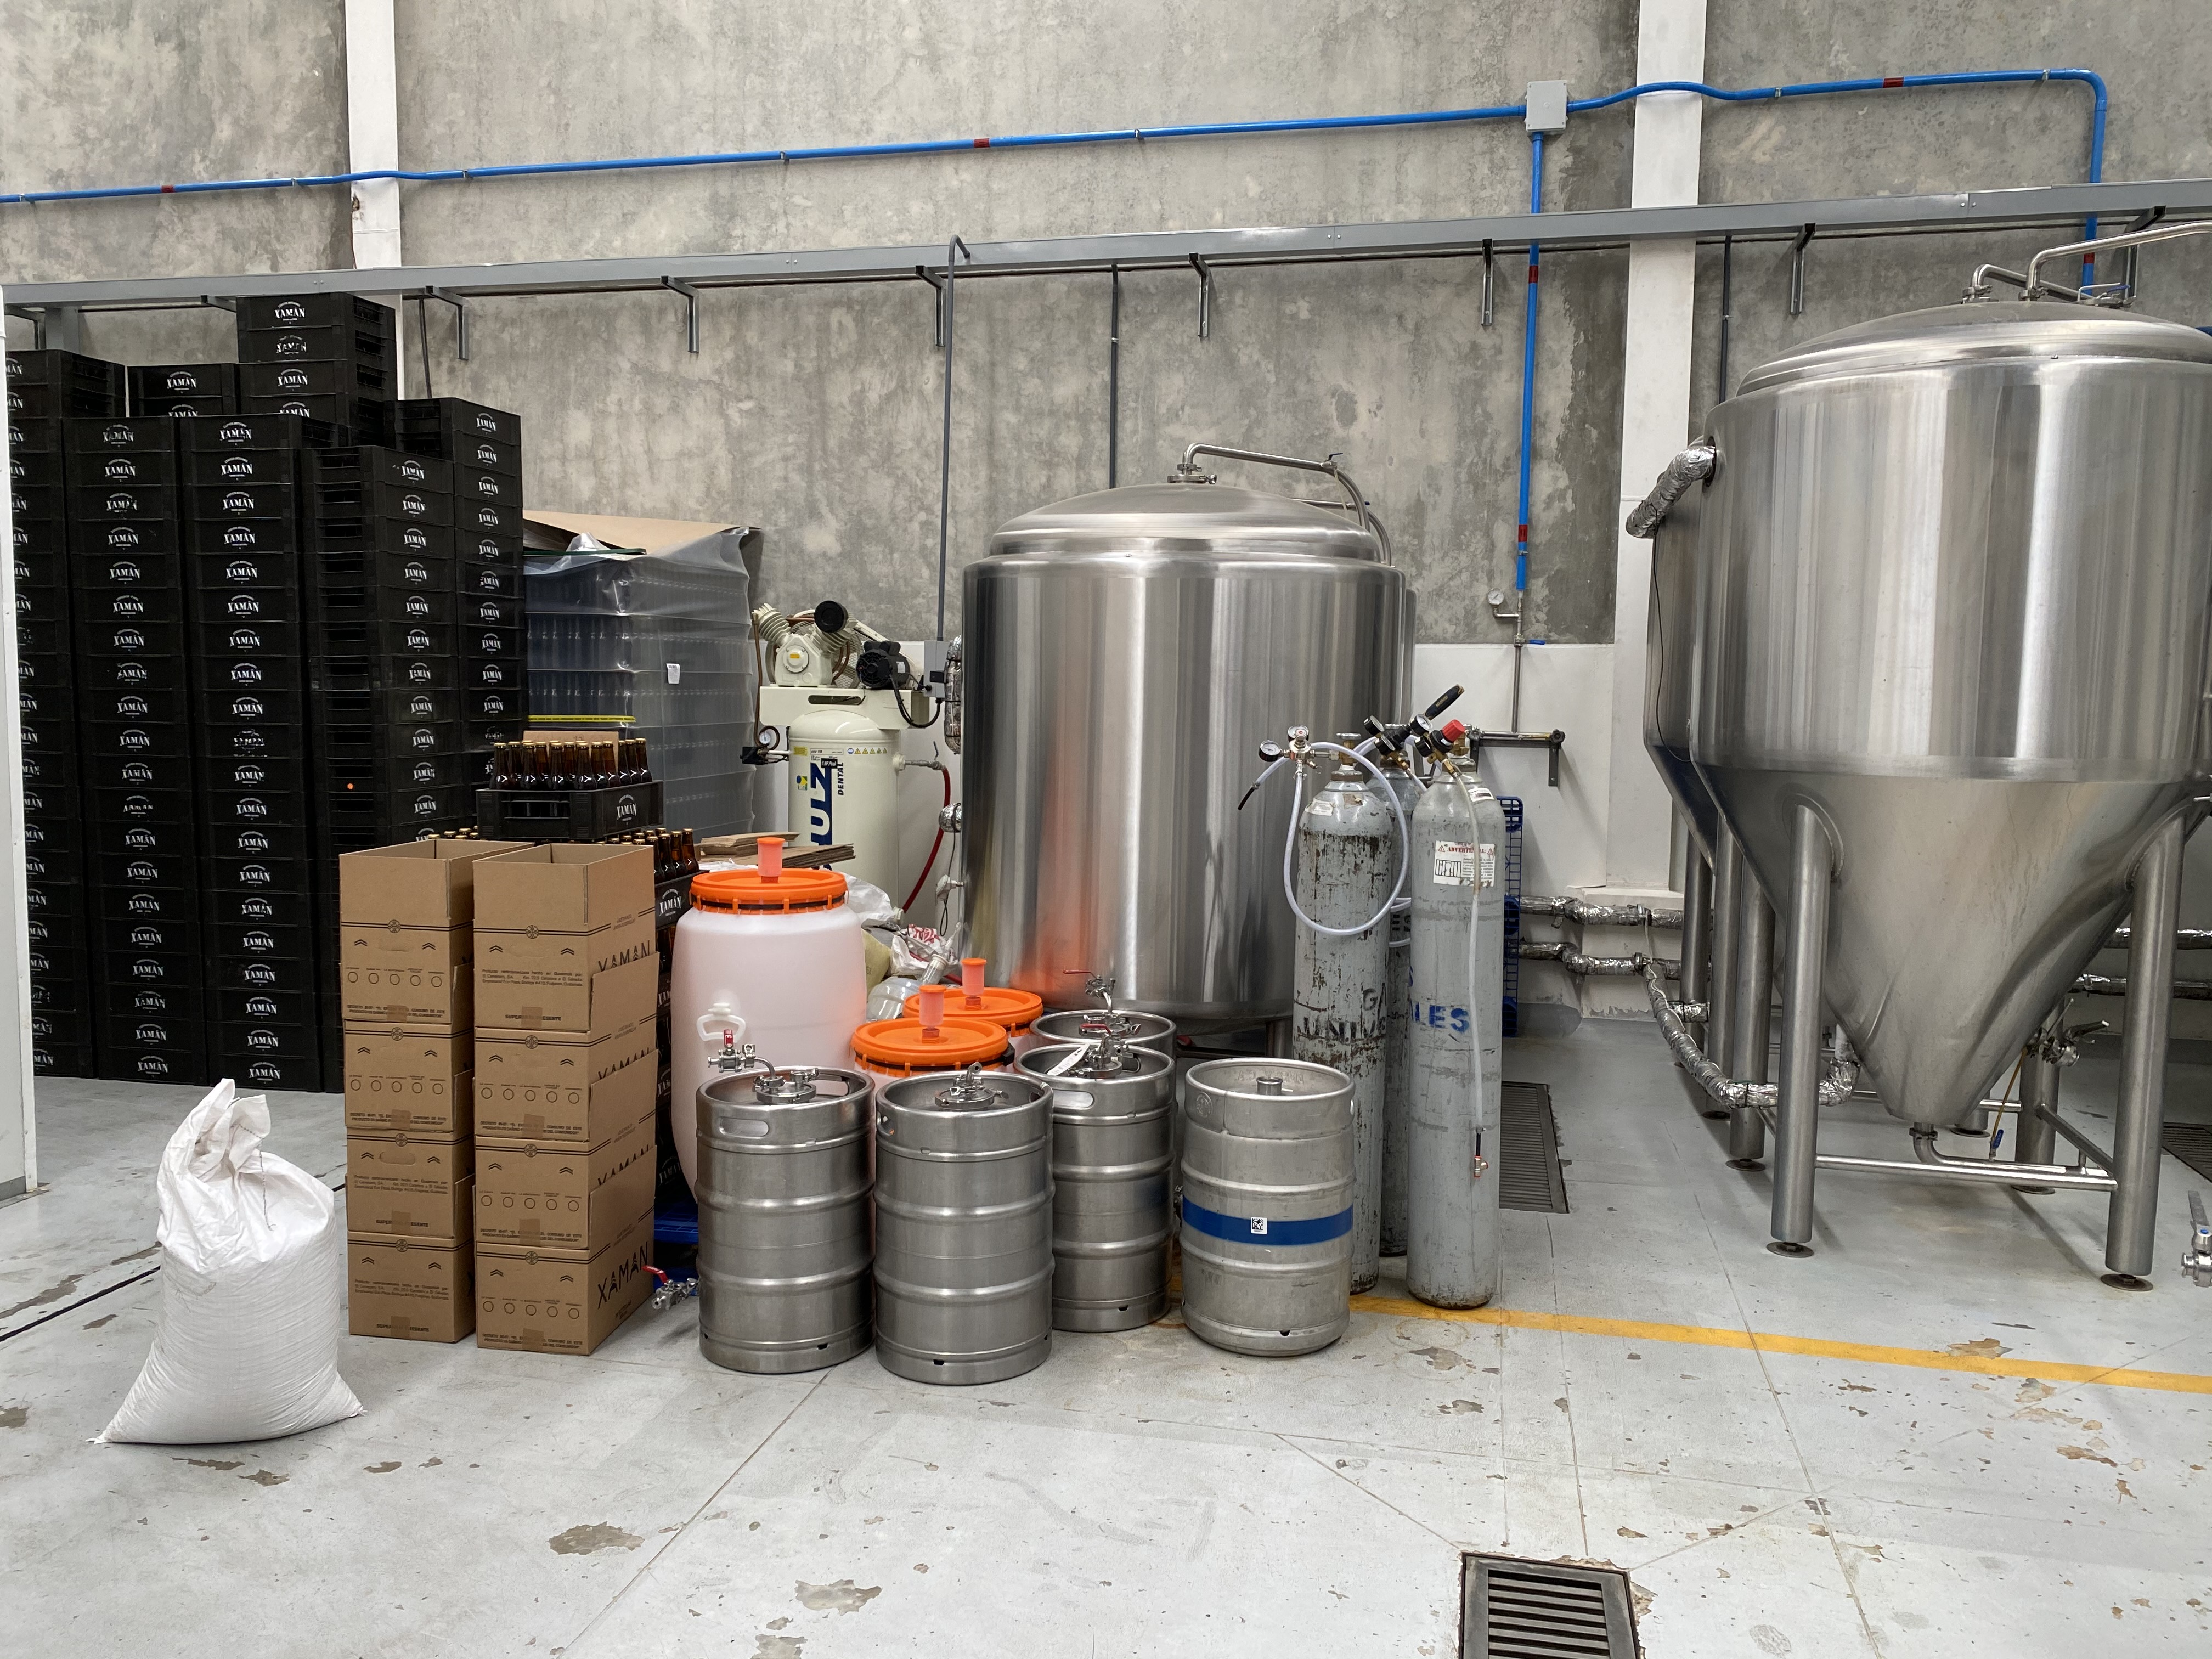
\includegraphics[width=8cm]{./img/IMG-7092.JPG}
    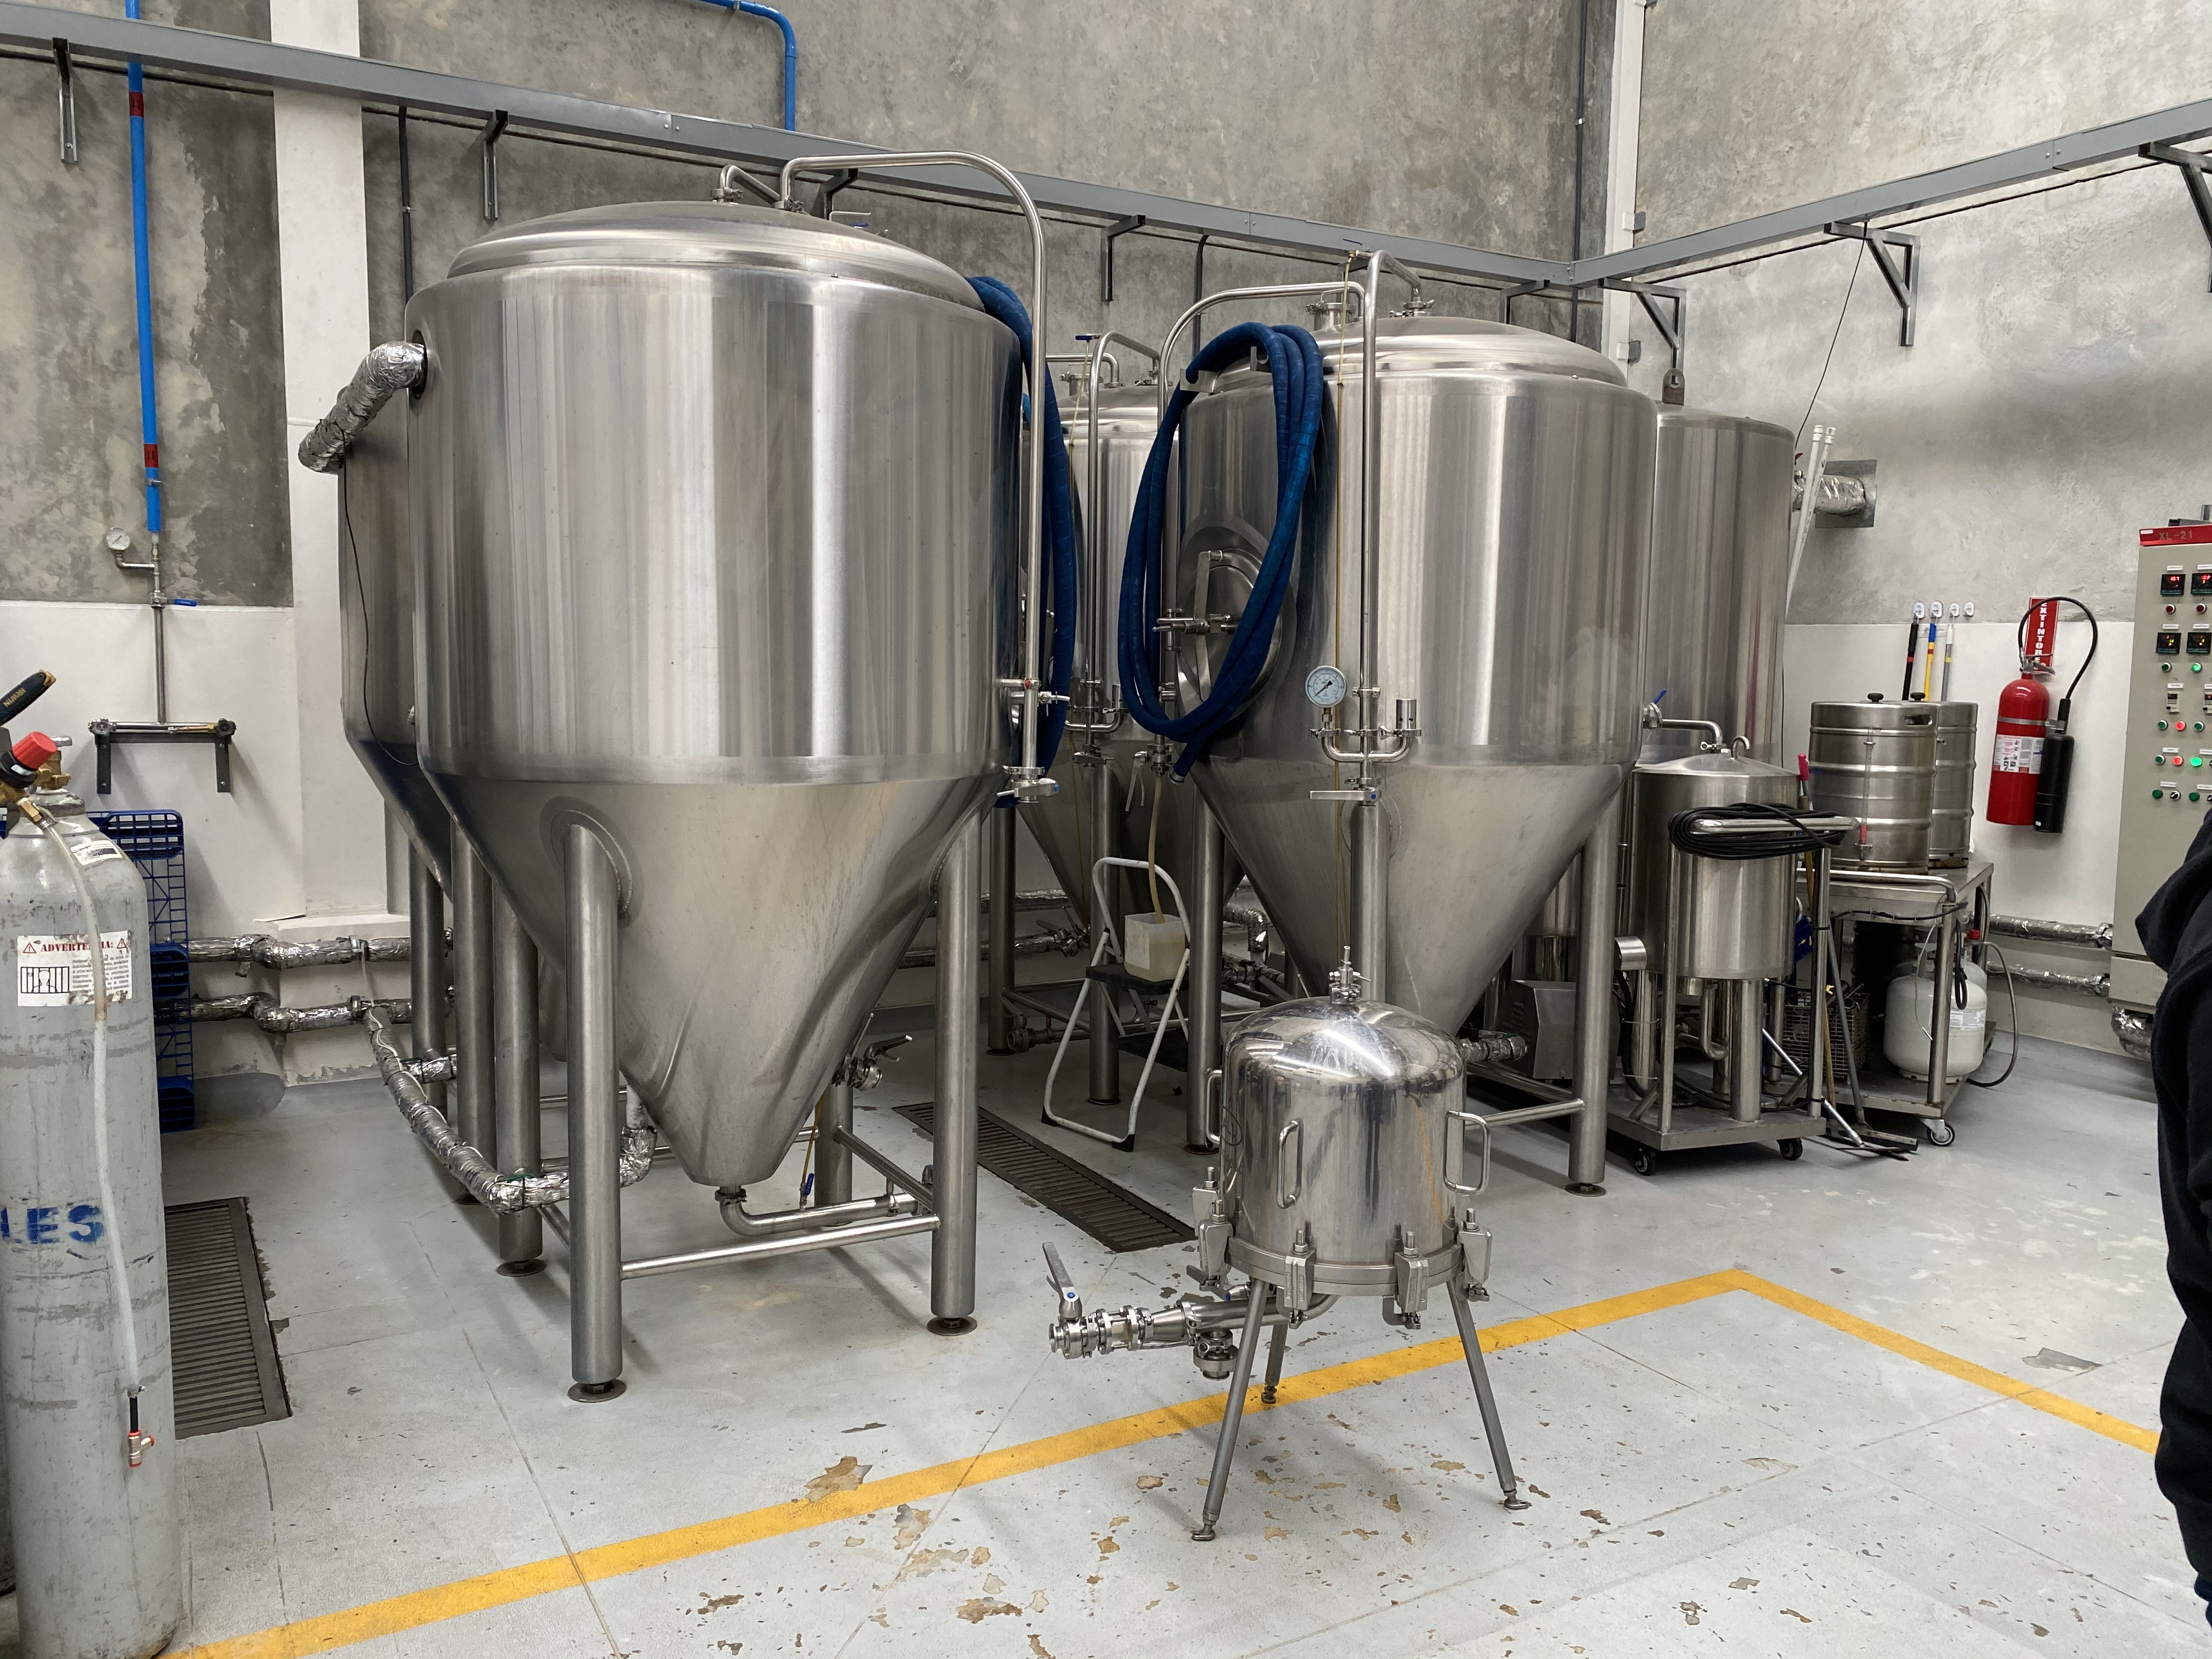
\includegraphics[width=8cm]{./img/IMG-7093.JPG}
    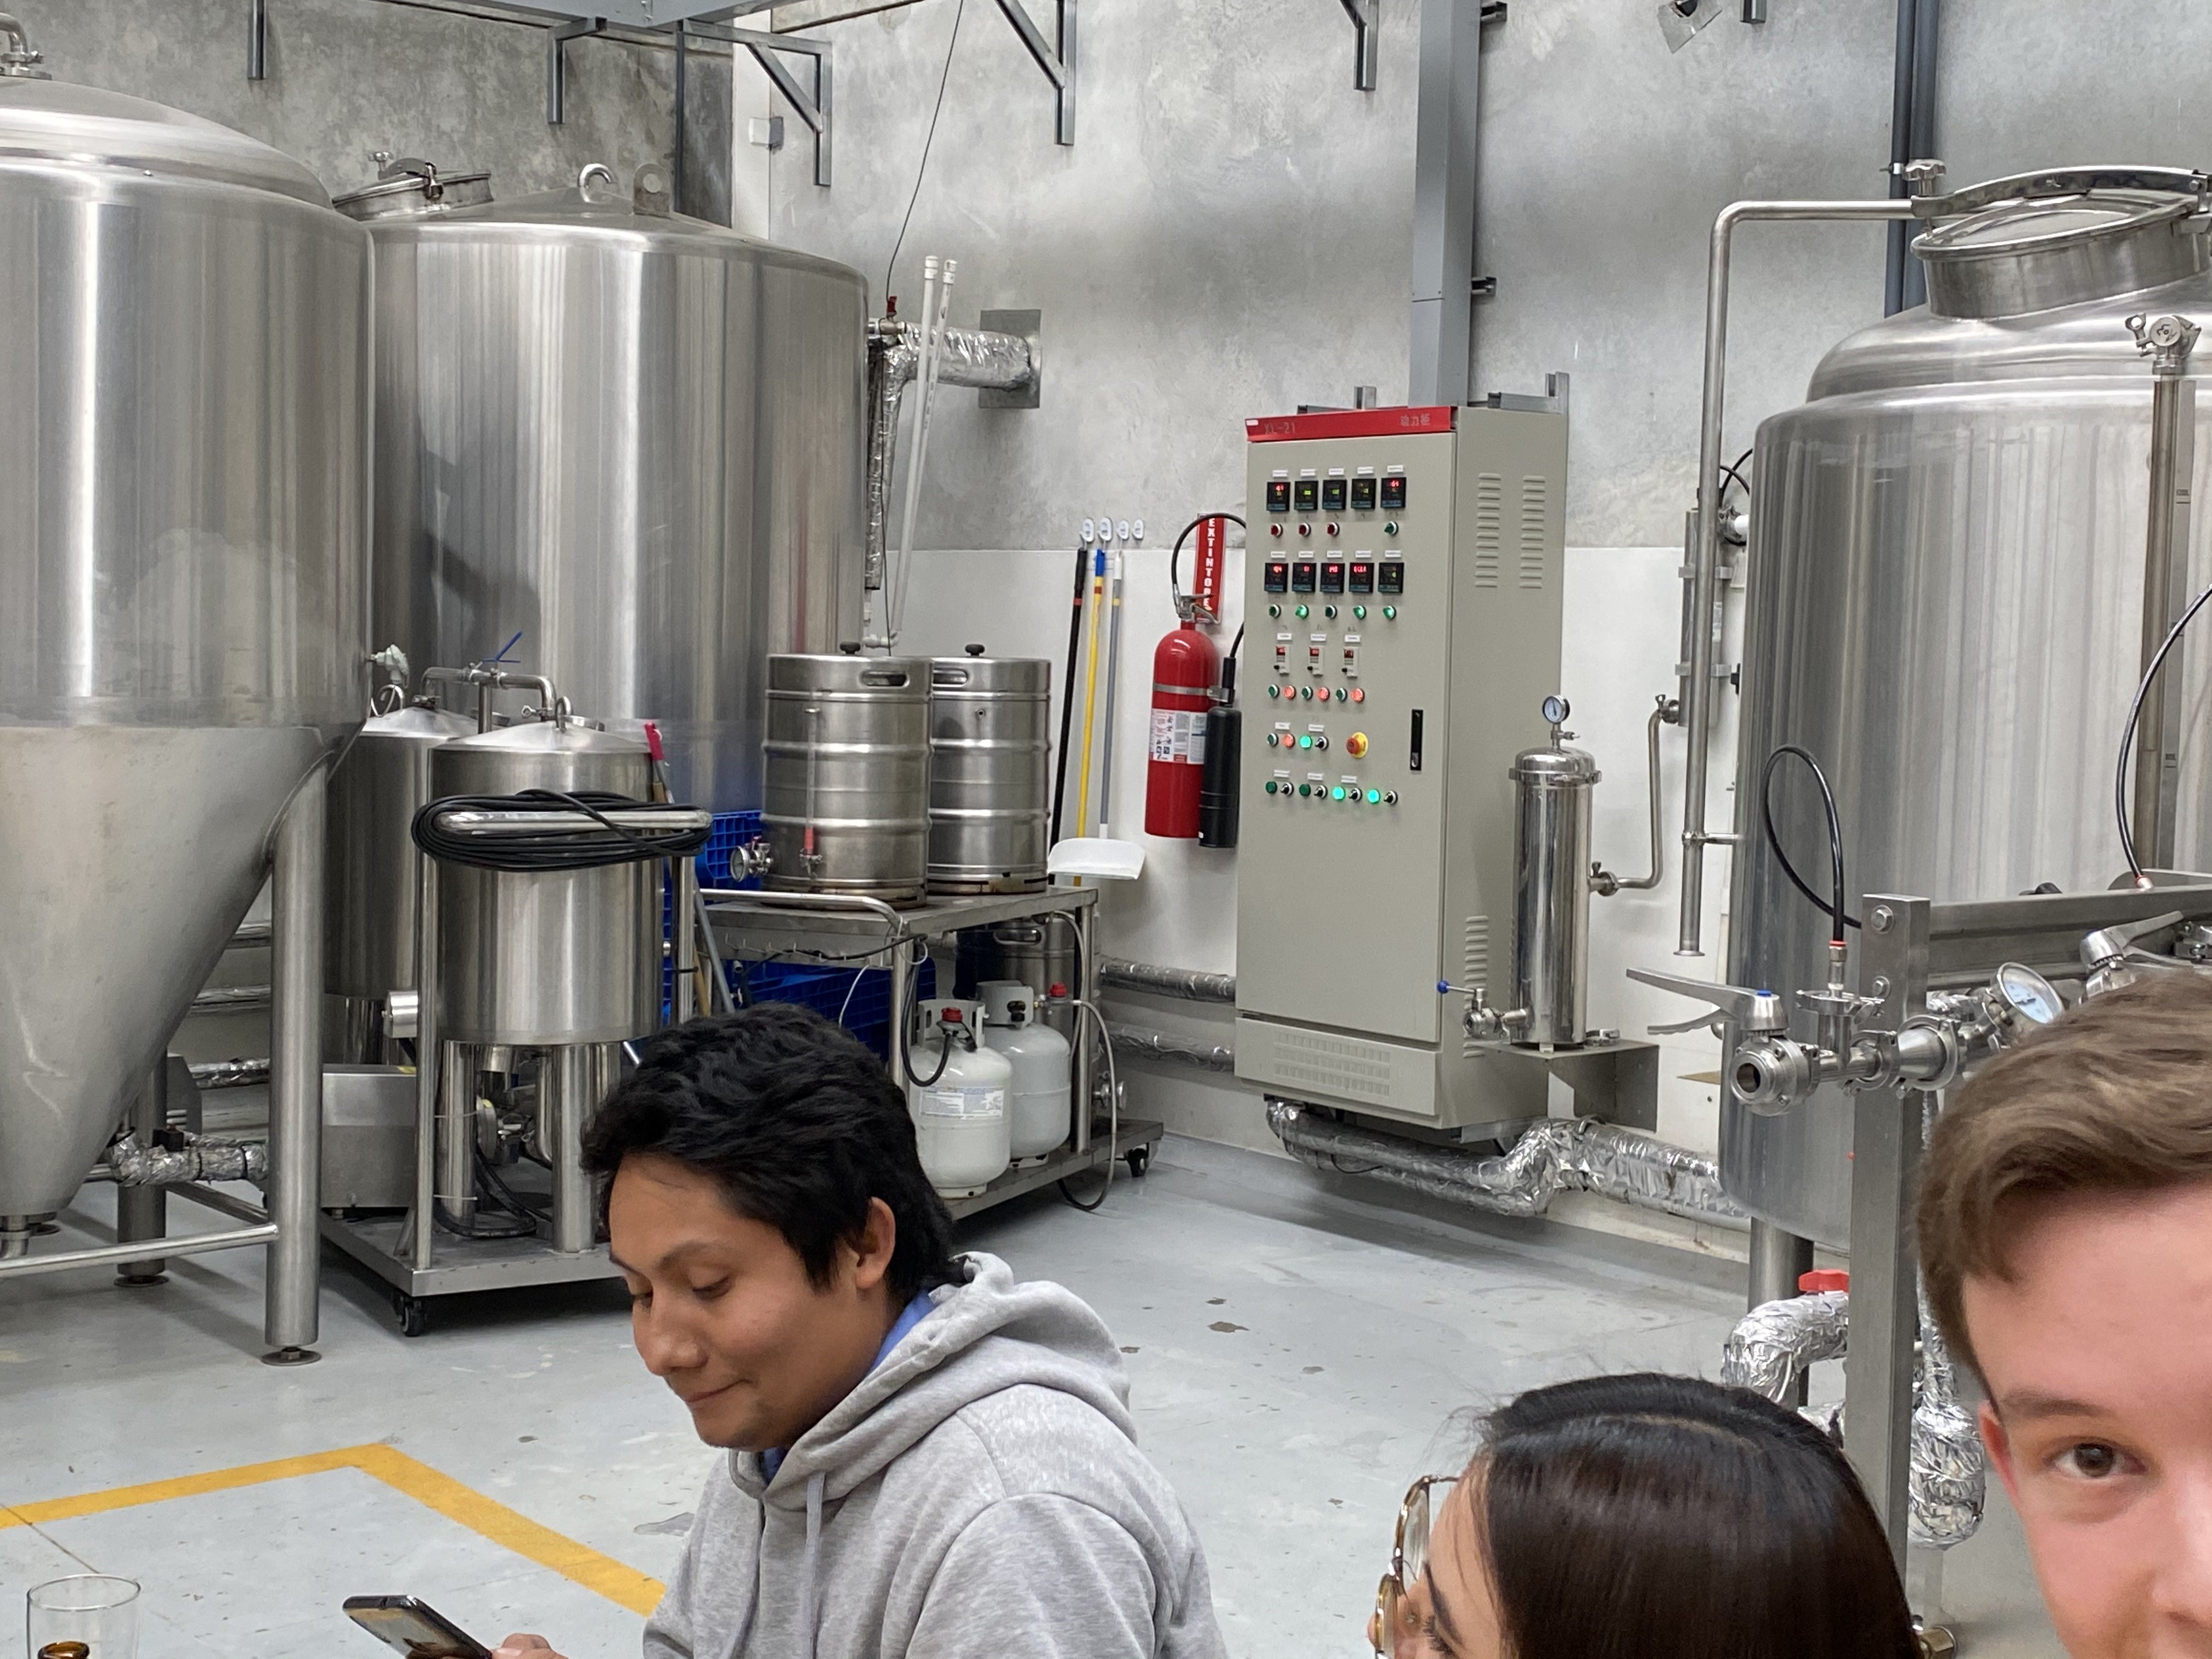
\includegraphics[width=8cm]{./img/IMG-7094.JPG}
    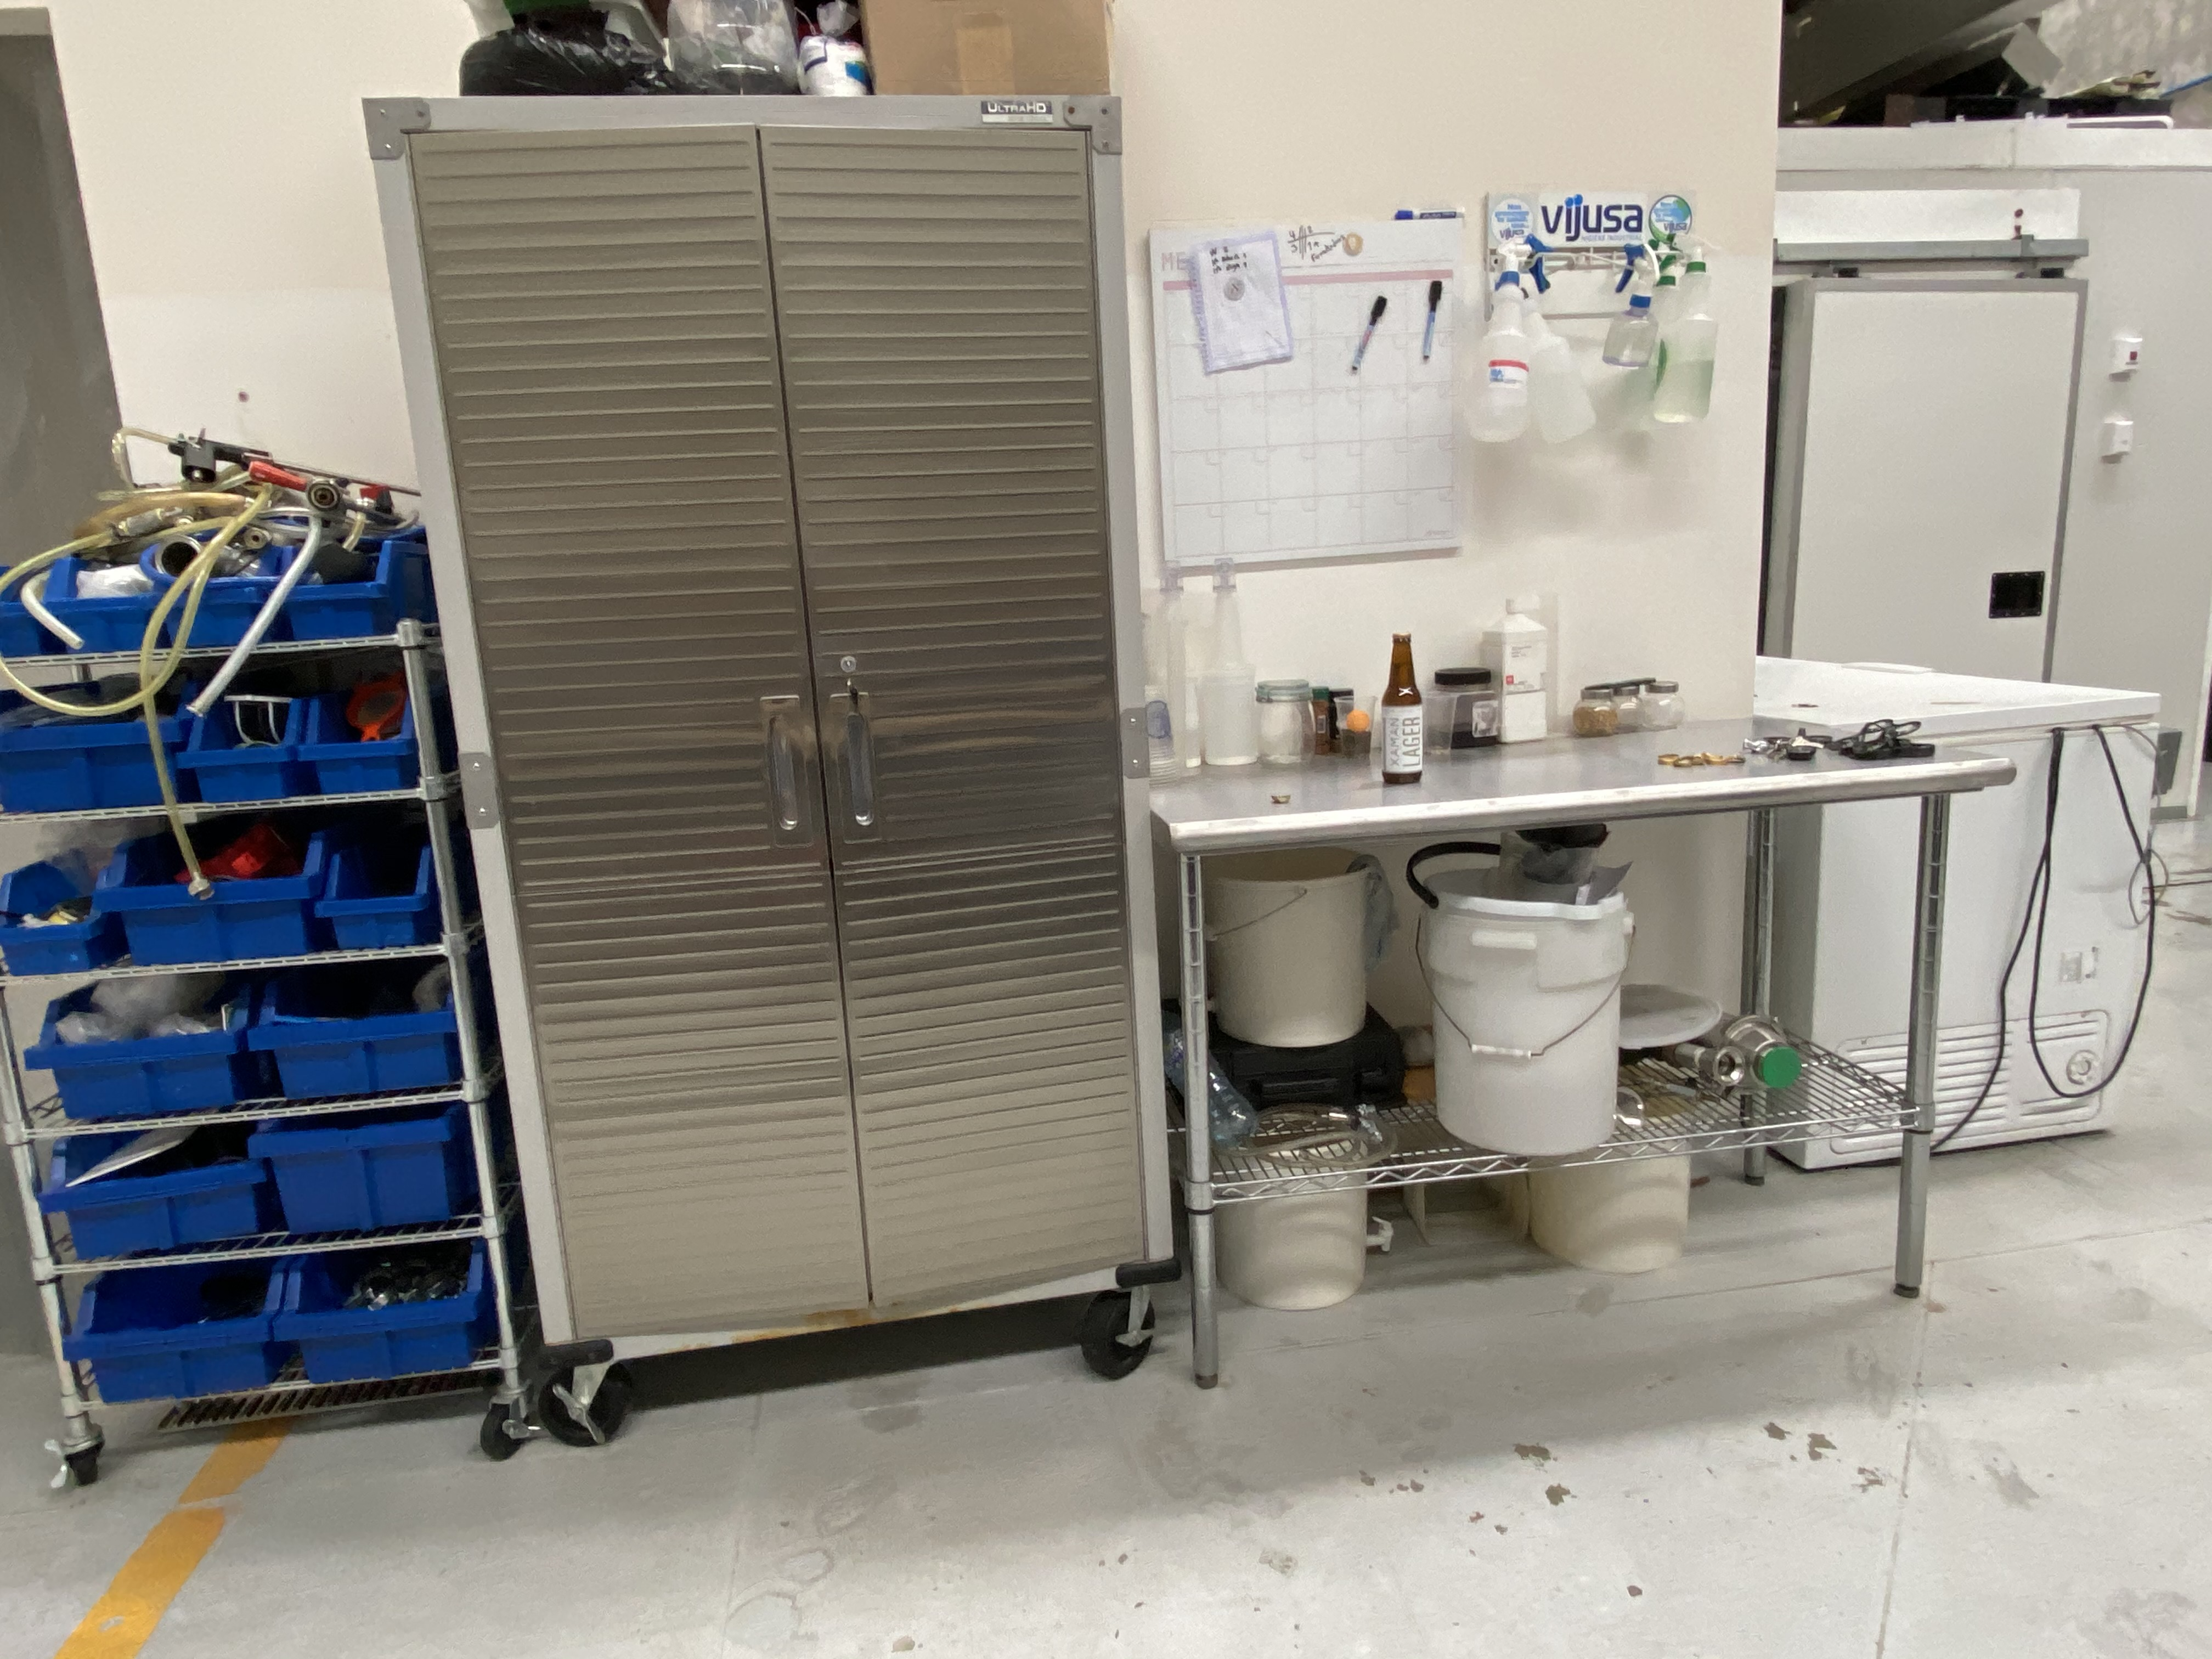
\includegraphics[width=8cm]{./img/IMG-7095.JPG}
    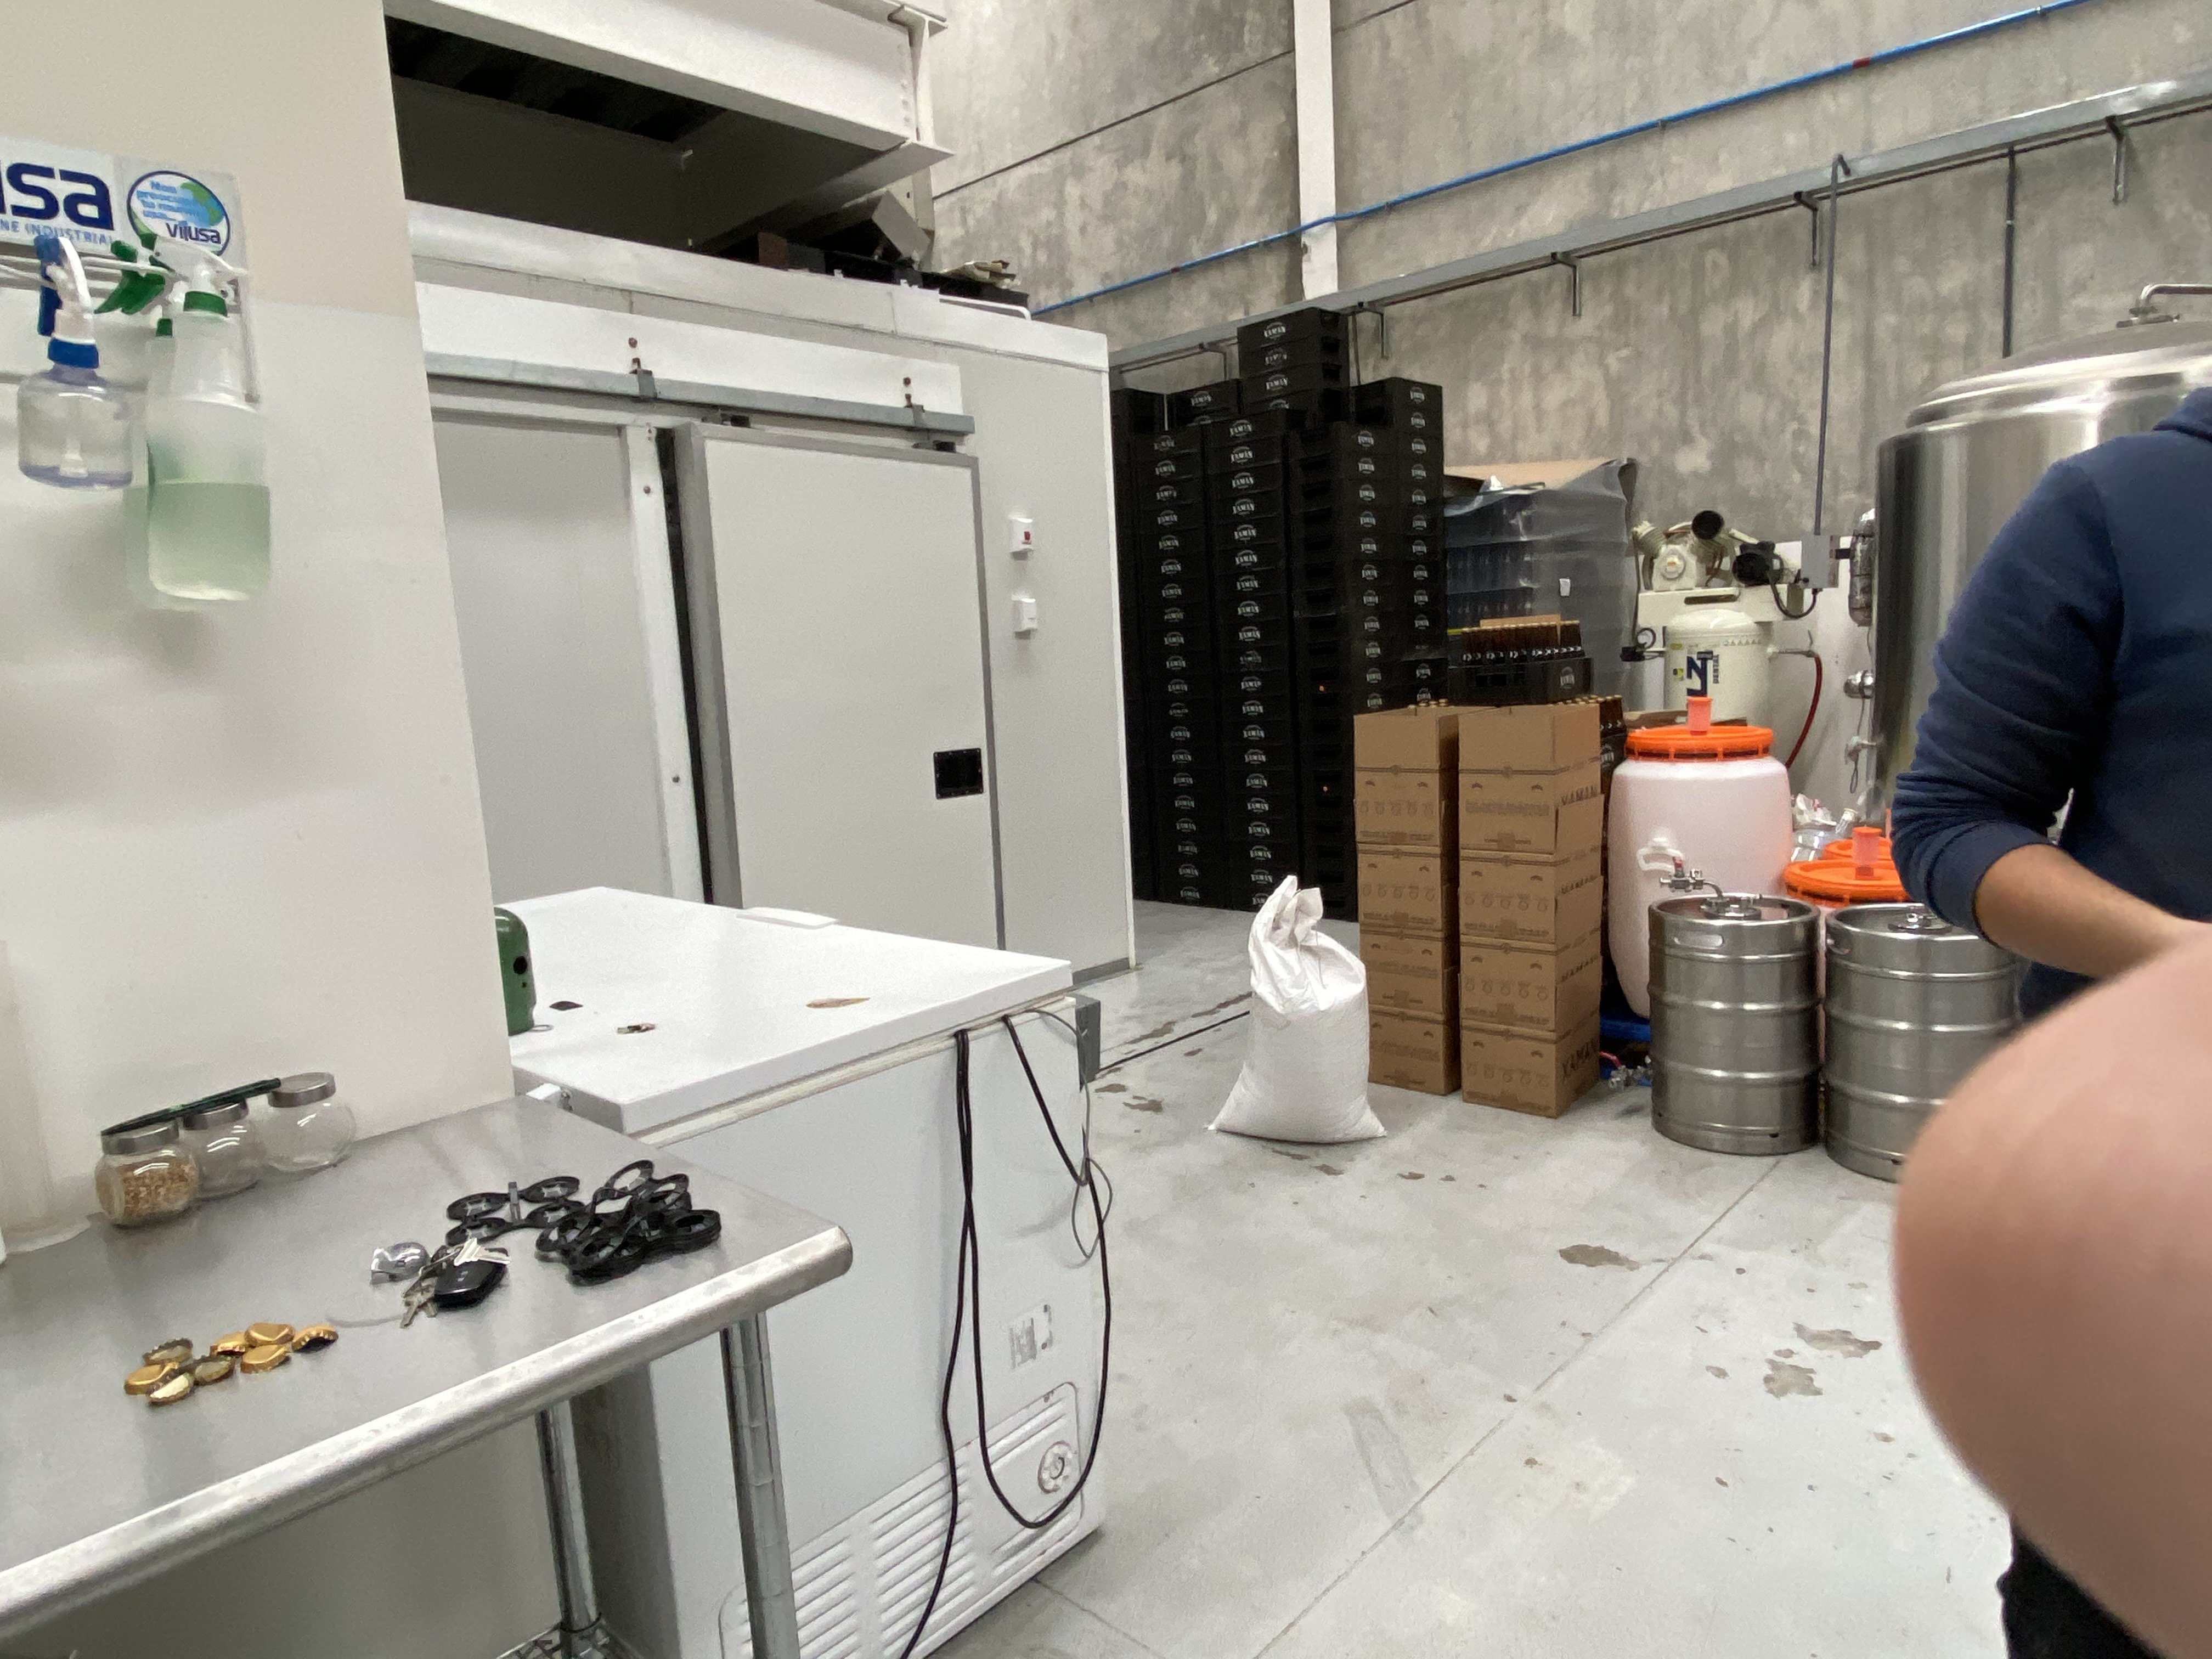
\includegraphics[width=8cm]{./img/IMG-7096.JPG}
    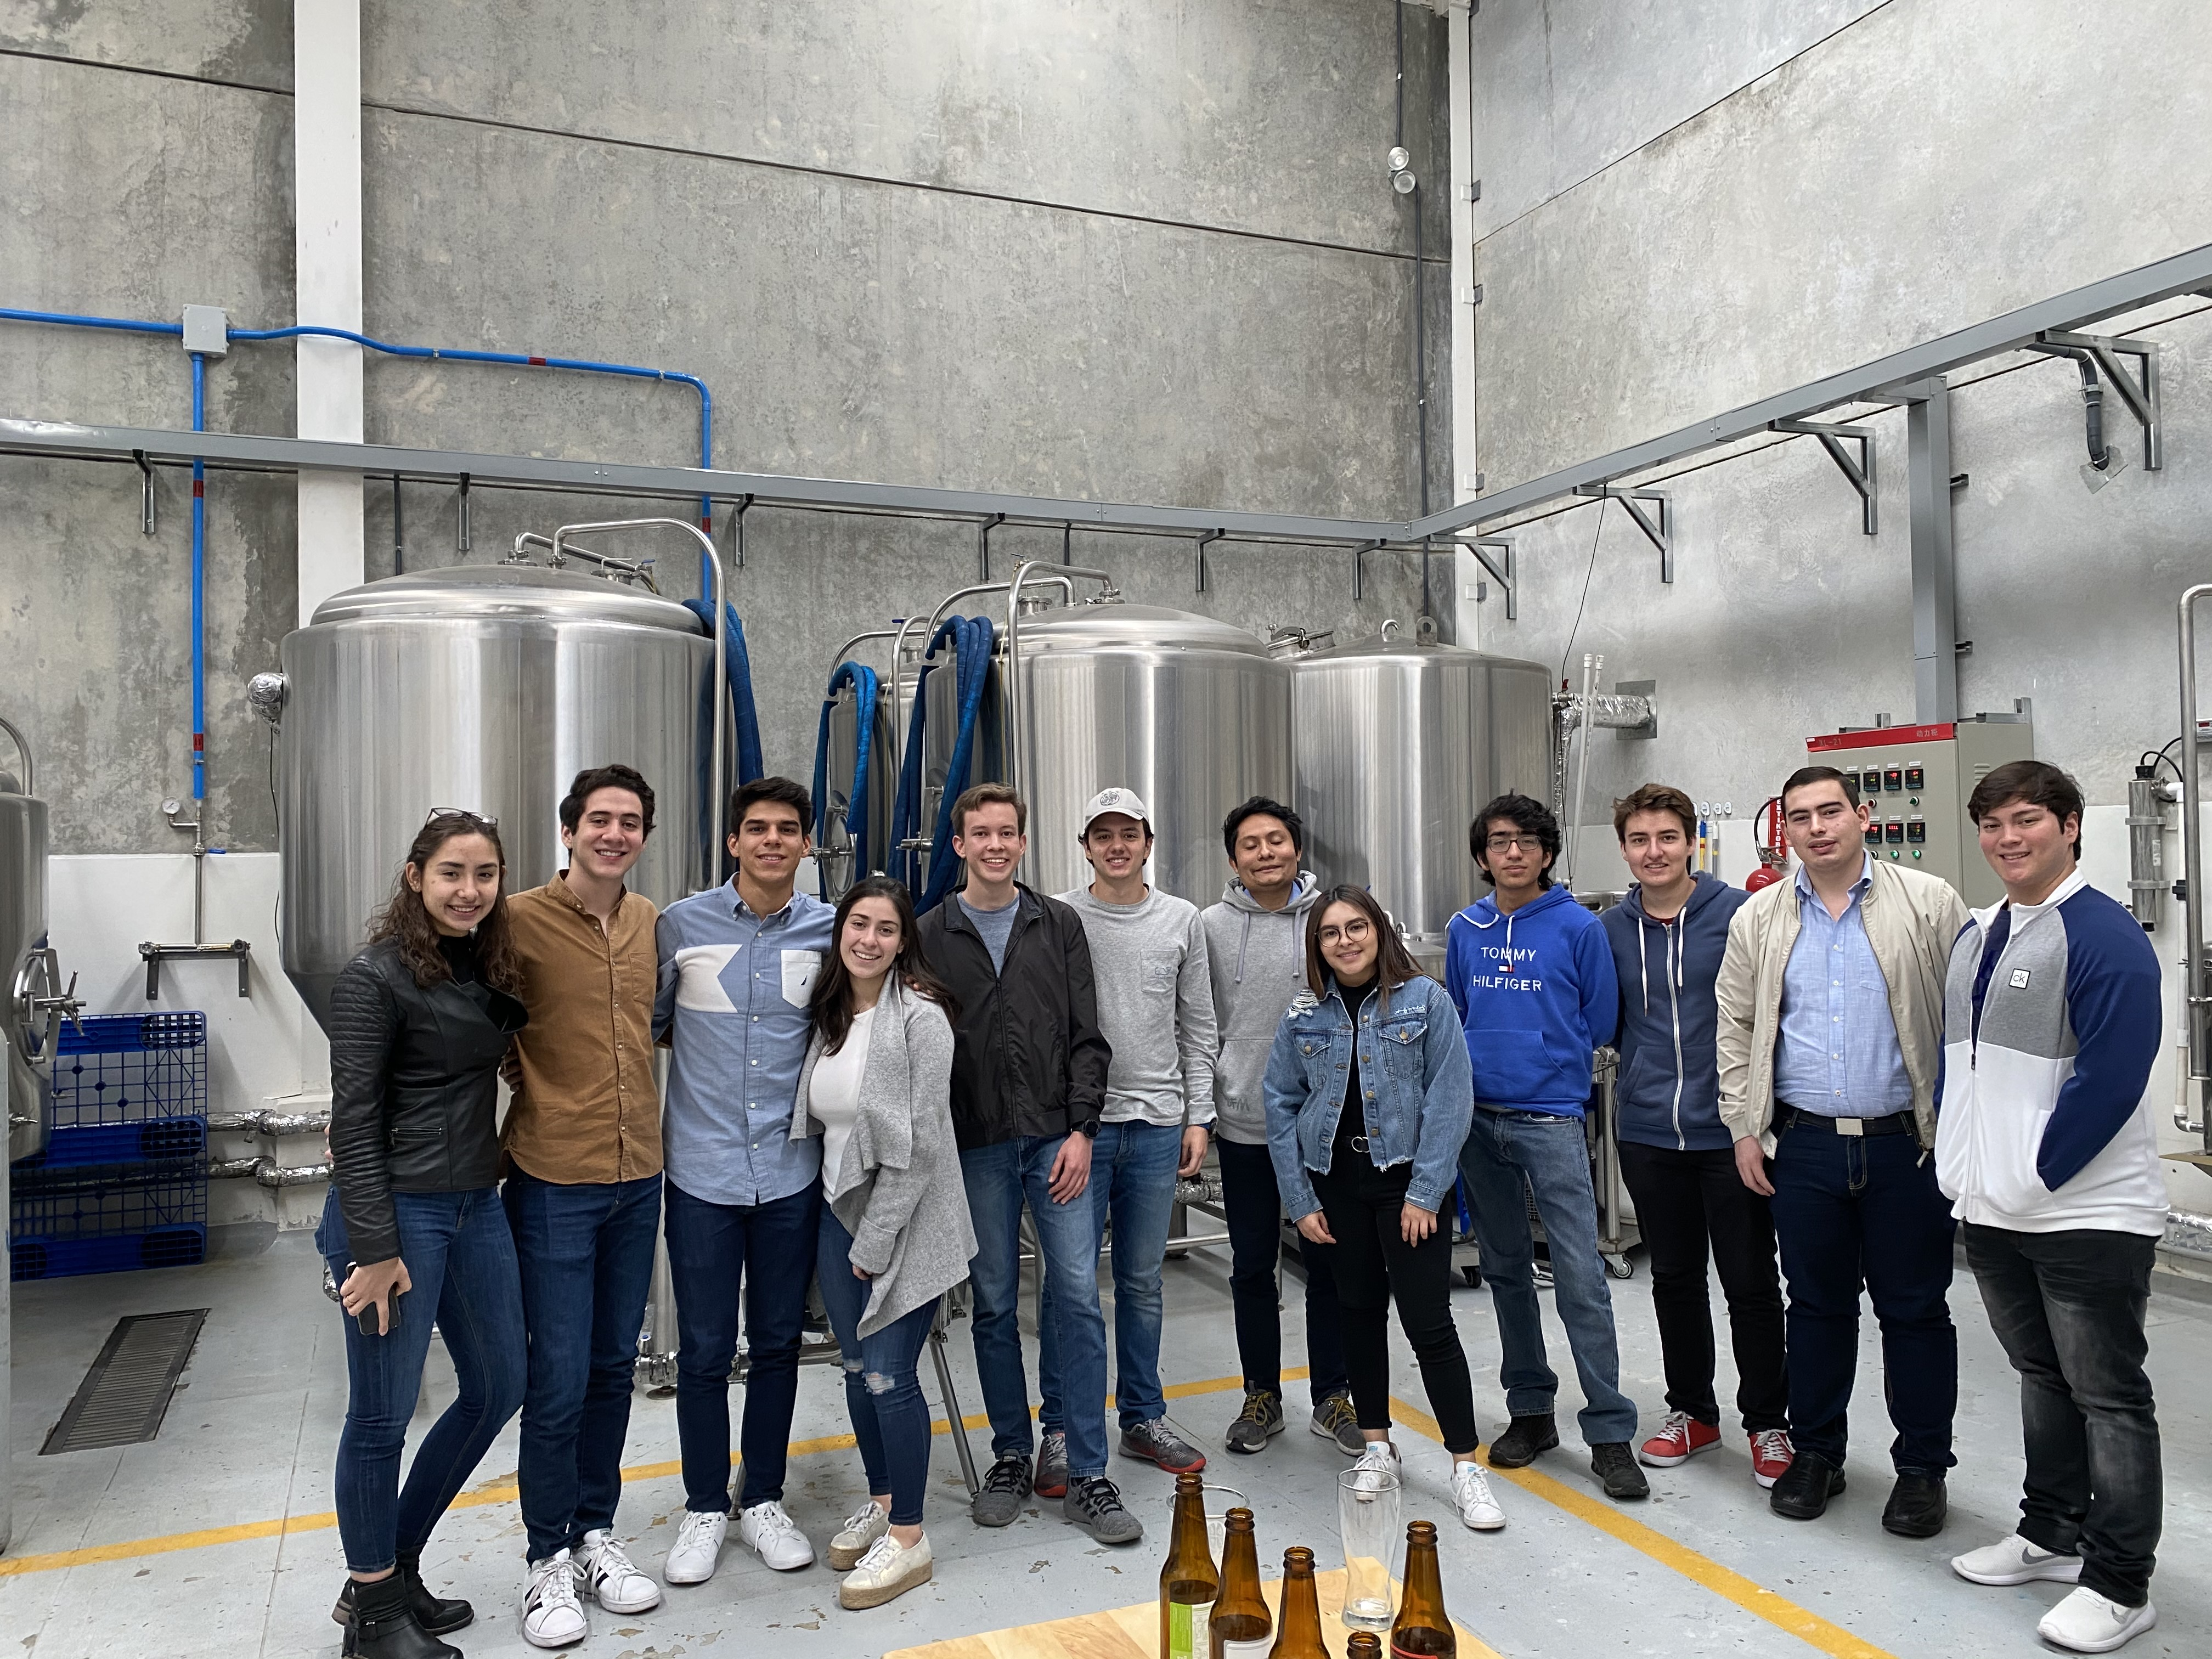
\includegraphics[width=8cm]{./img/IMG-7097.JPG}
    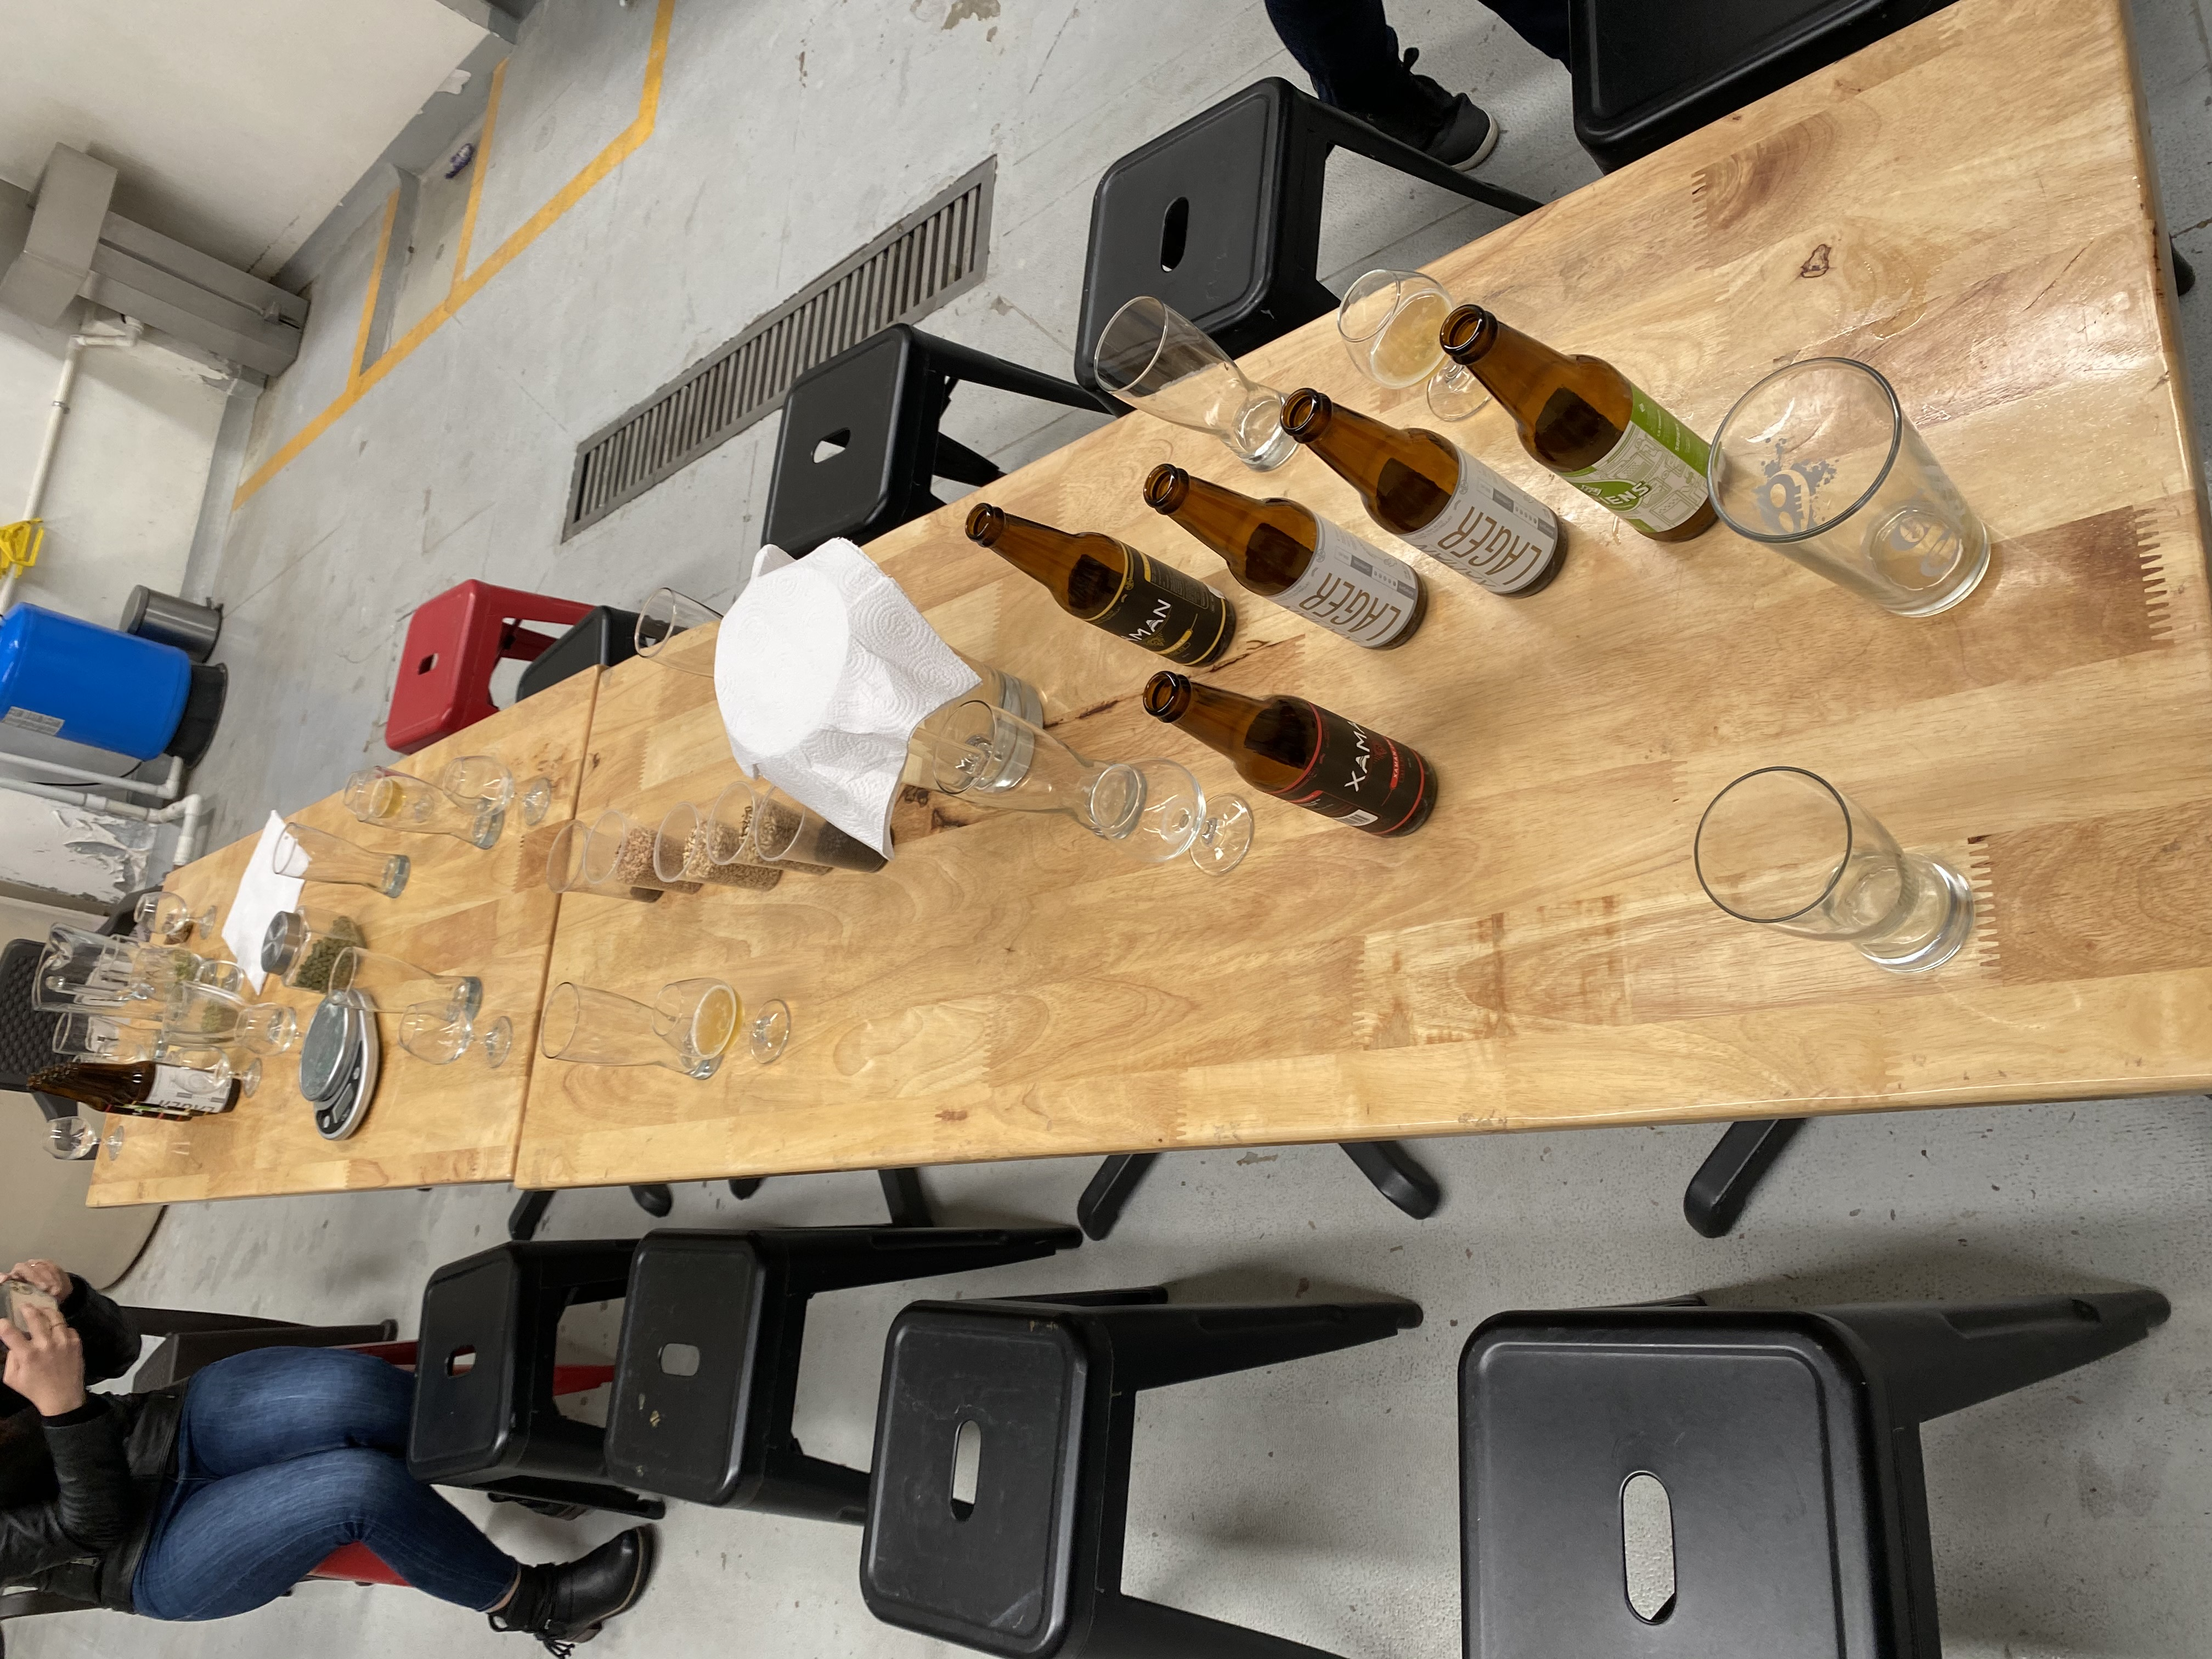
\includegraphics[width=8cm]{./img/IMG-7098.JPG}
    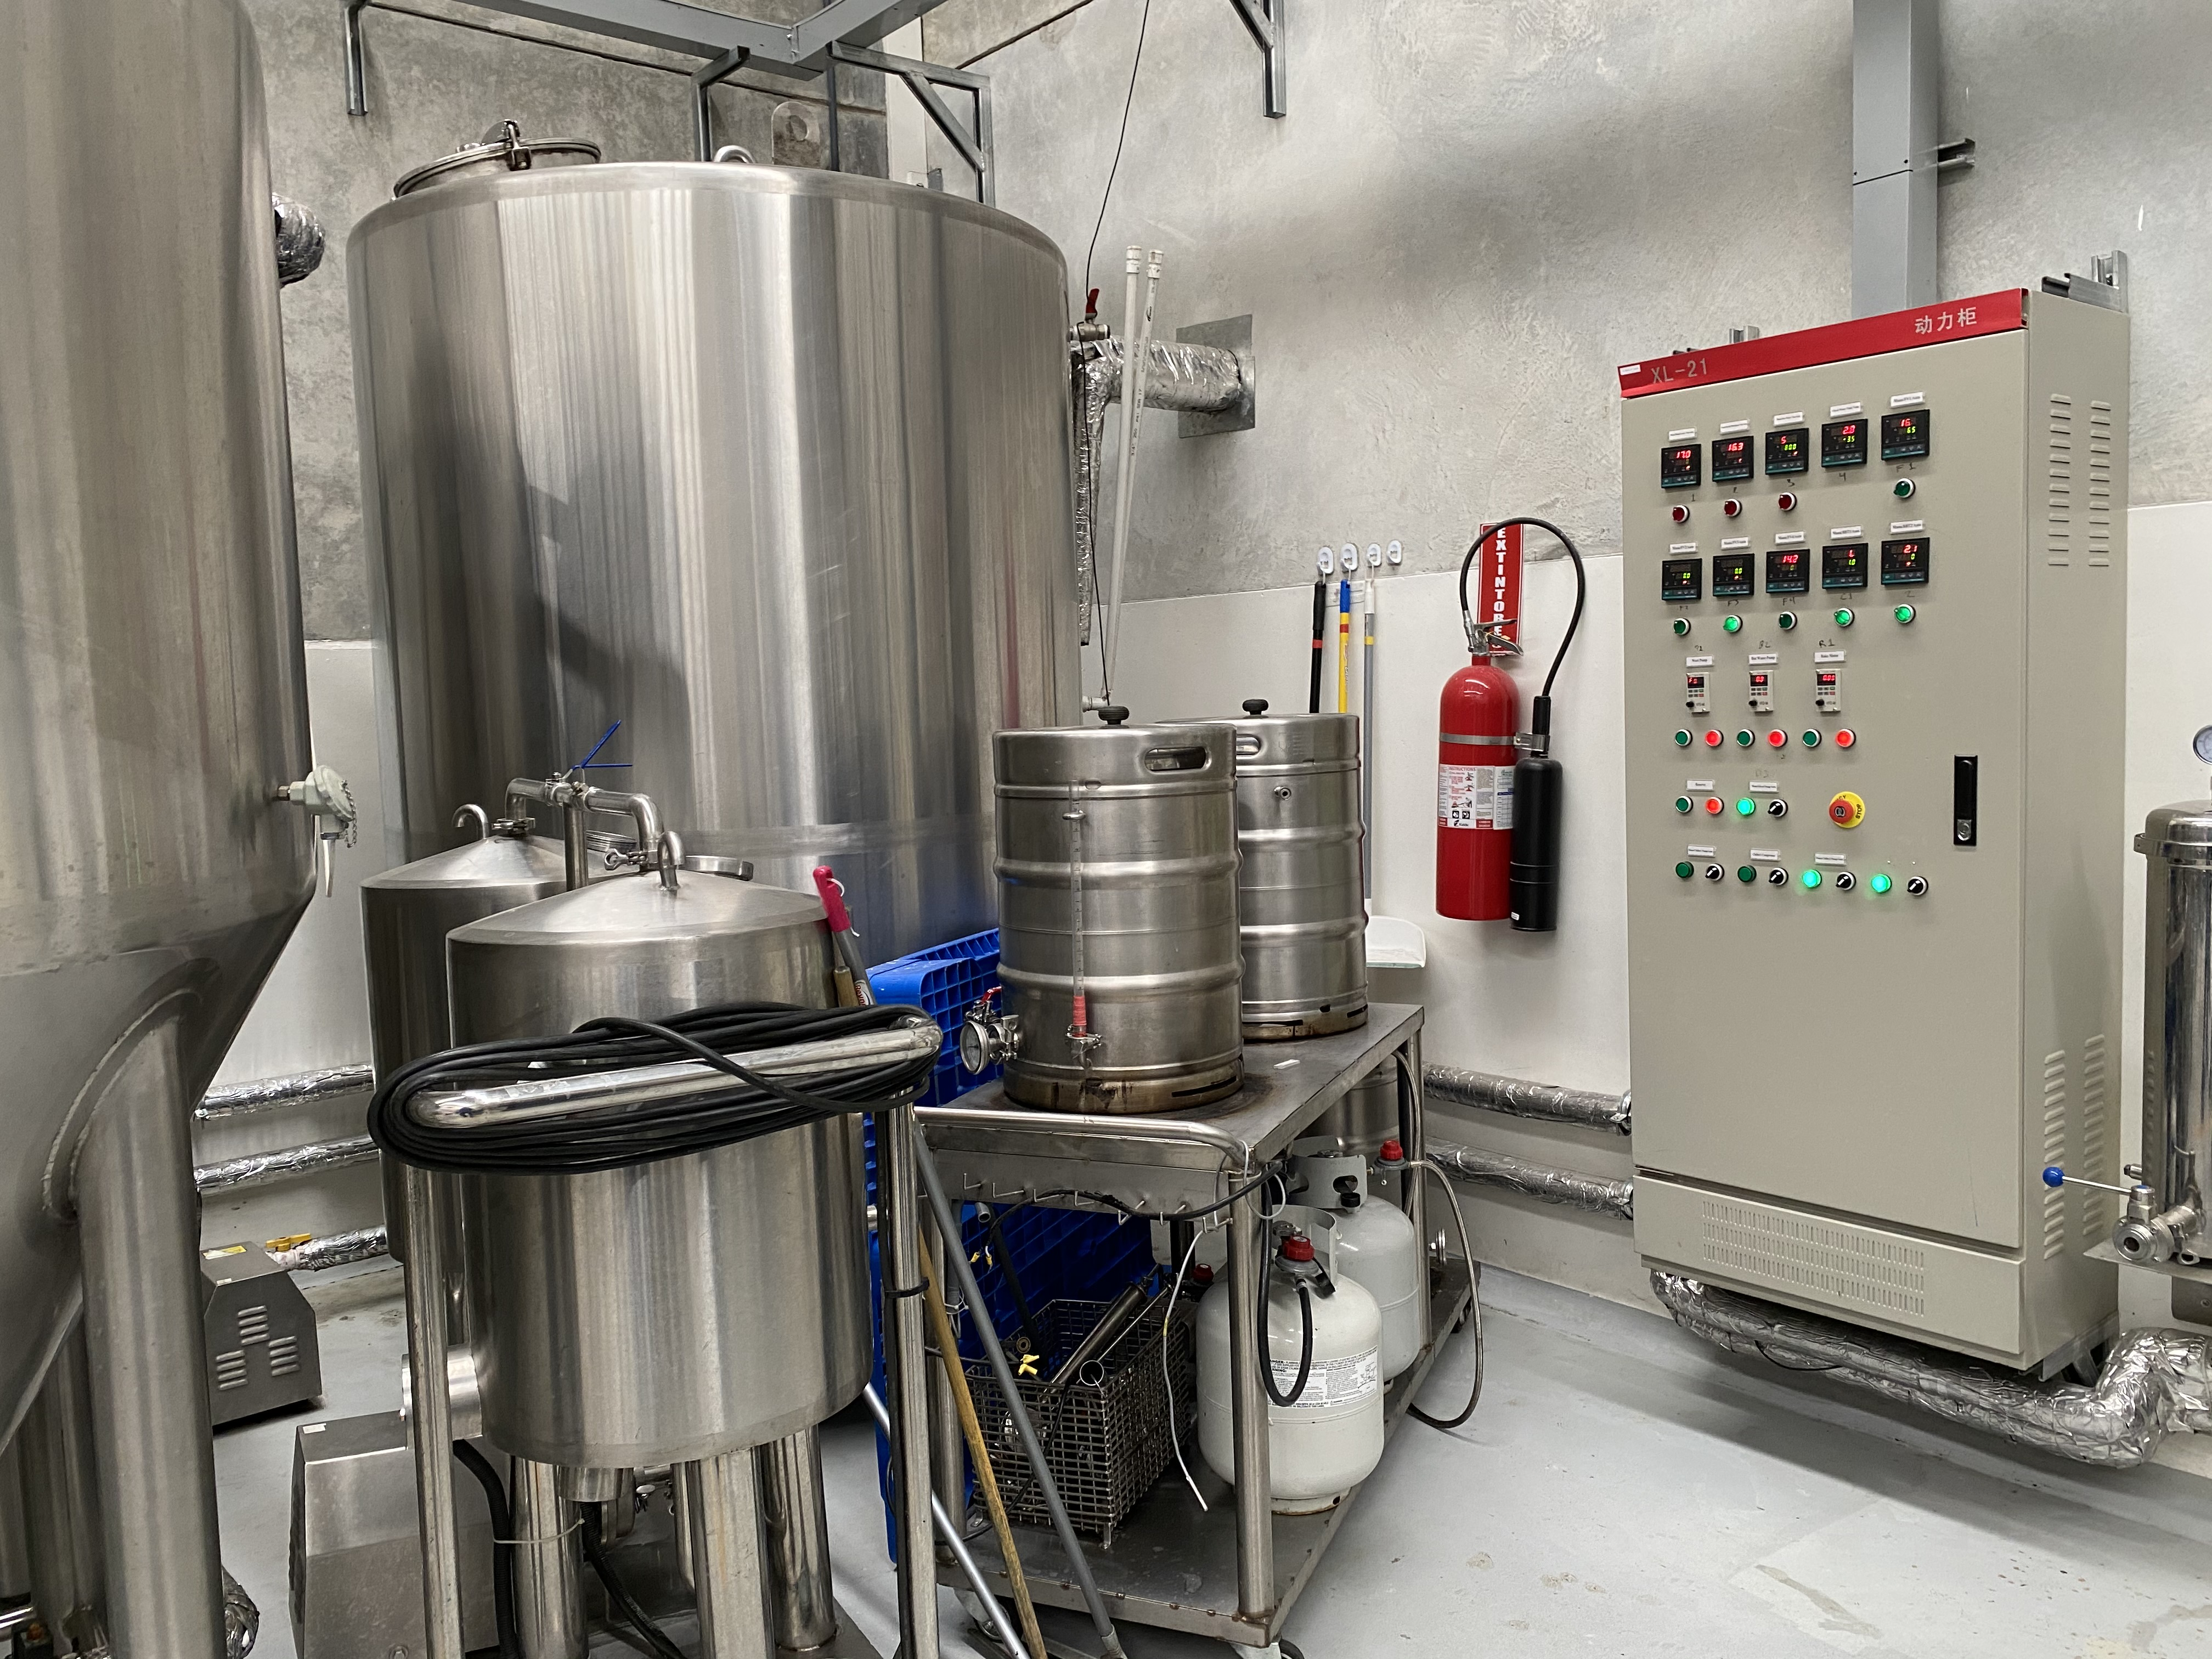
\includegraphics[width=8cm]{./img/IMG-7099.JPG}
    \caption{}
    \label{}
\end{figure}




\end{document}


